%
% Copyright (c) 2017  Zubax Robotics OU  <info@zubax.com>
%
% Distributed under BY-NC-ND (attribution required, non-commercial use only, no derivatives).
%

\documentclass{zubaxdoc}
\graphicspath{{document_templates/documentation_template_latex/}}

\usepackage{ConfigParamIndex}
\usepackage{amsmath}
\usepackage{textcomp}

\title{Zubax Babel Datasheet}

\hbadness=10000

\begin{document}
\frontmatter
\begin{titlepage}

\section*{Overview}

Zubax Babel is an advanced USB-\allowbreak{}CAN and UART-\allowbreak{}CAN adapter
that can be used as a standalone device or as an embeddable module for
OEM\footnote{Original equipment manufacturer.}.

Babel uses the quasi-standard SLCAN (aka LAWICEL) protocol (with Zubax extensions)
for transferring CAN data over USB and UART.
There is a wide selection of software products that can communicate with SLCAN-compatible adapters.

\section*{Features}

\begin{itemize}
    \item Very low latency -- the cumulative latency between the host system
          and the CAN bus is under 1 millisecond.\footnote{Tested via USB on Linux 3.13
          using a low-latency SLCAN driver from the PyUAVCAN library.}

    \item Very high throughput -- the device handles more than 5000 frames per second in either direction
          continuously.\footnote{Tested via USB on Linux 3.13.
          When using the UART interface, the throughput is limited by the UART baud rate setting.}

    \item Large RX buffer (255 CAN frames plus 2KB of serial buffers) allows the device to handle short-term
          traffic bursts regardless of the throughput of the host-side interface.

    \item Proper prioritization of the outgoing CAN frames.
          The adapter properly schedules the outgoing frames, avoiding the inner priority inversion problem
          in the TX queue.

    \item Embedded 120~$\Omega{}$ CAN bus termination resistor that can be turned on and off by a command.

    \item Embedded CAN bus power supply output that can be turned on and off by a command.

    \item CAN bus supply voltage monitoring.

    \item SMD soldering pads for OEM applications.
\end{itemize}

\BeginRightColumn

\section*{Applications}

\begin{itemize}
    \item General-purpose USB-CAN or UART-CAN adapter.
    \item Diagnostic, monitoring, and development tool for \href{http://uavcan.org}{UAVCAN} networks.
          We recommend the UAVCAN GUI Tool for use with UAVCAN applications.
    \item Generic CAN/UAVCAN development board.
    \item Programmable CAN unit in OEM applications.
\end{itemize}

\centering{
    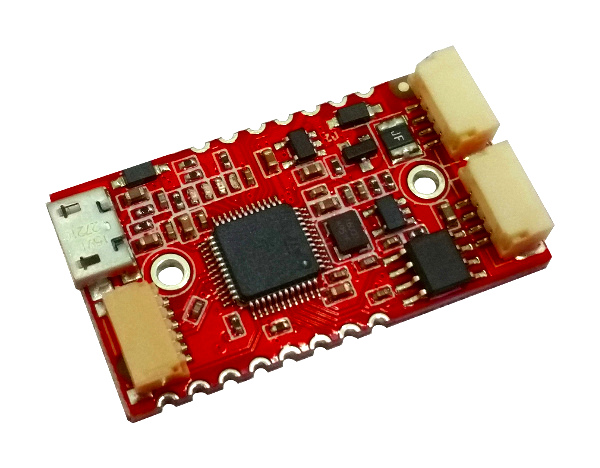
\includegraphics[width=0.45\textwidth]{top}
    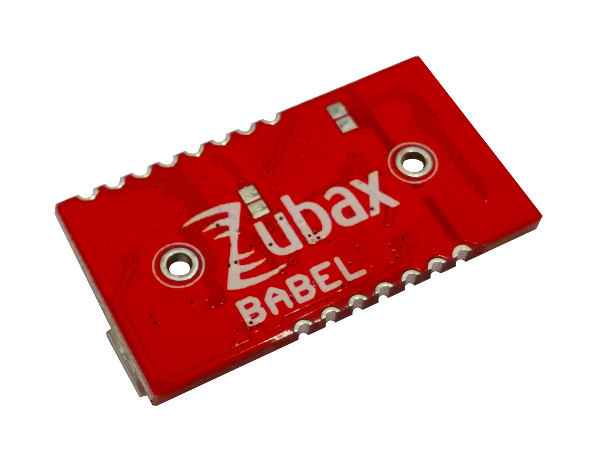
\includegraphics[width=0.45\textwidth]{bottom}
}

\end{titlepage}

\tableofcontents
\BeginRightColumn
\listoffigures
\BeginRightColumn
\listoftables

\mainmatter

\chapter{Overview}

Zubax Babel is an advanced USB-CAN and UART-CAN adapter
that can be used as a standalone device or as an embeddable module for
OEM.

\section{Accessories}

Babel can be used with the following accessories:
\begin{itemize}
    \item Plastic enclosure described in the section \ref{sec:enclosure}.
    \item UAVCAN cabling and related items.
    \item Standard USB cables.
    \item Cables compatible with the Dronecode Autopilot Connector Standard.
\end{itemize}

Please contact your supplier for the ordering information.

\subsection{Enclosure}\label{sec:enclosure}

Babel can be enclosed in a plastic enclosure pictured on the figure \ref{fig:enclosure}.
The enclosure provides a mechanical protection that makes the device more suitable for use as a
general-purpose desktop CAN adapter tool.

\begin{figure}[hb]
    \centering
    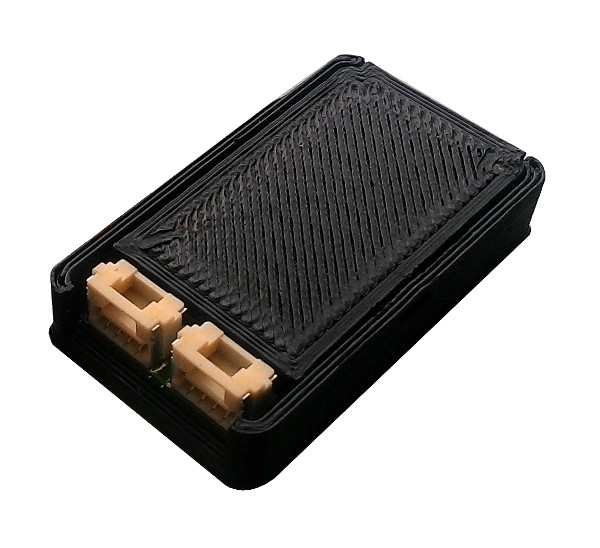
\includegraphics[width=0.45\textwidth]{housing}
    \caption{Plastic enclosure.\label{fig:enclosure}}
\end{figure}

Please contact your supplier for the ordering information;
alternatively, visit the website at \mbox{\url{https://github.com/Zubax/zubax_babel}} to download
the 3D-printable enclosure models suitable for in-house manufacturing.

\section{Quality assurance}

Every manufactured Babel undergoes an automated testing procedure that validates that
the device is functioning as designed.
The test log for every manufactured device is available on the web at
\url{https://device.zubax.com/device_info}.
This feature can be used to facilitate the traceability of purchased devices and
provide additional safety assurances.

Every manufactured device has a strong digital signature stored in its non-volatile memory
which proves the origins of the product and eliminates the risk of sourcing unlicensed or
counterfeit hardware.
This signature is referred to as Certificate of Authenticity (CoA).
Please refer to the \href{https://kb.zubax.com}{Zubax Knowledge Base} to learn more about
the certificate of authenticity and how it can be used to trace the origins of your hardware.

\chapter{Characteristics}

\section{Absolute maximum ratings}

Stresses that exceed the limits specified in this section may cause permanent damage to the device.
Proper operation of the device within the limits specified in this section is not implied.

\begin{ZubaxSimpleTable}{Absolute maximum ratings}{|c X|c c|c|}
    Symbol            & Parameter                & Min  & Max & Unit \\
    $V_\text{supply}$ & Supply voltage           & -0.3 & 6   & V \\
    $T_\text{oper}$   & Operating temperature    & -40  & 85  & \degree{}C \\
                      & UART RX input voltage    & -0.3 & 6   & V\\
                      & CAN H/L input voltage    & -4   & 16  & V\\
\end{ZubaxSimpleTable}

\section{Environmental conditions}

\begin{ZubaxTableWrapper}{Environmental conditions}
    \begin{ZubaxWrappedTable}{|c X|l c|c|c|}
        Symbol            & Parameter                     &  Min & Max & Unit \\
        $T_\text{oper}$   & Operating temperature         & -40  & 85  & \degree{}C \\
        $T_\text{stor}$   & Storage temperature           & -40  & 85  & \degree{}C \\
        $\phi_\text{oper}$& Operating humidity\tnote{a}   & 0    & 100 & \%RH\\
    \end{ZubaxWrappedTable}
    \begin{tablenotes}
        \item[a] Condensation not permitted.
    \end{tablenotes}
\end{ZubaxTableWrapper}

\section{Power supply}\label{sec:power}

Babel requires a +5 V DC power supply input
which can be delivered via any of the available interface connectors.

The device has a reverse current protection on the USB power input
which prevents back-powering the USB host when it is turned off.

The CAN power output has a solid state switch that can be enabled and disabled
by setting the configuration parameter \CfgRef{can.power+on}.
The device can always be powered from the CAN bus regardless of the state of the power switch.

An additional +3.3 V DC output on the SMD pads can be used to power any external circuitry when the device
is used as a development board or in OEM applications.
The pinout specification for the SMD pads is provided in the section \ref{sec:smd_pads}.

The topology of the power supply circuits is documented on the figure \ref{fig:power_supply_scheme}.
Power input and output capabilities per interface are summarized in the table \ref{table:power_supply_summary}.

\begin{figure}[!hbt]
    \centerline{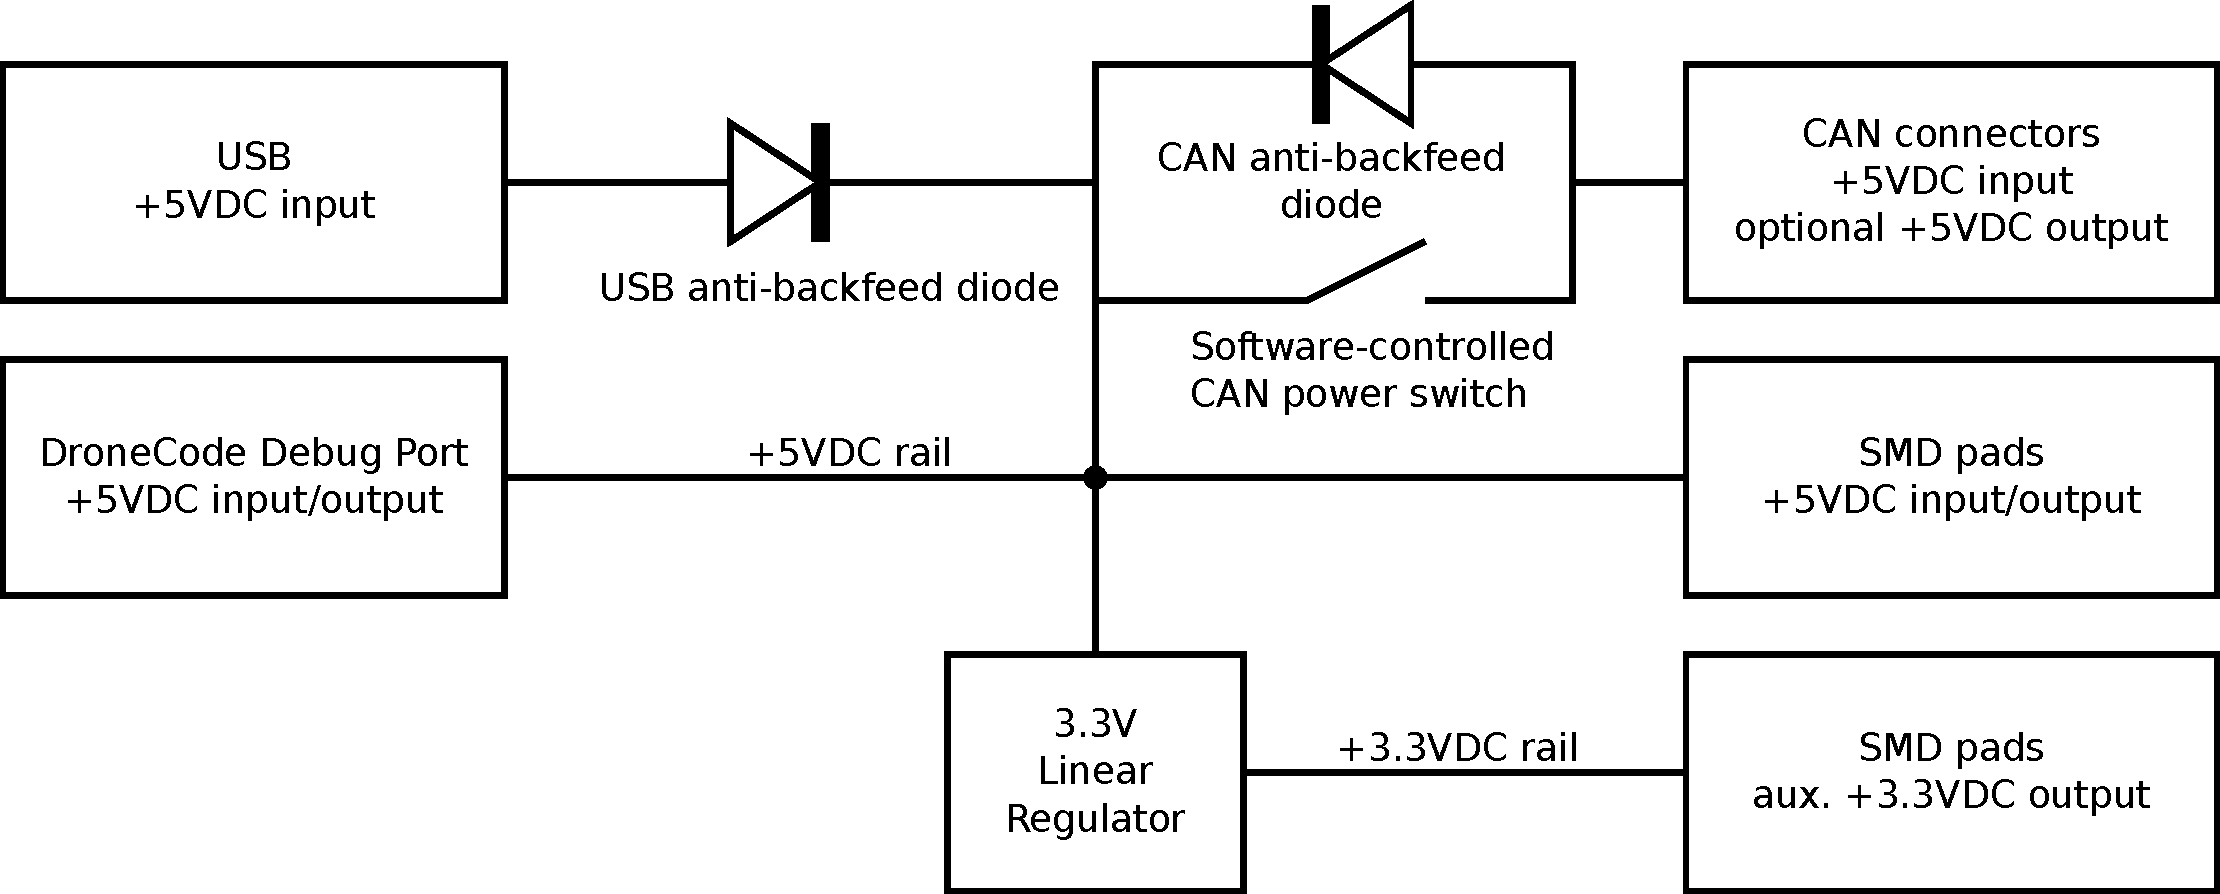
\includegraphics[width=1\textwidth]{power_supply}}
    \vspace{1em}
    \caption{Power supply architecture.\label{fig:power_supply_scheme}}
\end{figure}

\begin{ZubaxSimpleTable}{Power supply summary}{|l X X|}\label{table:power_supply_summary}
    Interface            & Direction              & Section \\
    CAN                  & Input, optional output & \ref{sec:can_bus} \\
    USB                  & Input                  & \ref{sec:usb} \\
    Dronecode debug port & Input, output          & \ref{sec:dronecode_debug_port} \\
    SMD pads             & Input, output          & \ref{sec:smd_pads} \\
\end{ZubaxSimpleTable}

\begin{ZubaxTableWrapper}{Power supply characteristics}
    \begin{ZubaxWrappedTable}{|c X| c c c | c|}\label{table:power}
        Symbol            & Parameter                       & Min & Typ & Max & Unit \\
        $V_\text{supply}$ & Supply voltage\tnote{a}         & 4.0 & 5.0 & 5.5 & V  \\
        $I_\text{supply}$ & Self power consumption\tnote{b} & 30  & 50  & 80  & mA \\
        $I_\text{total}$  & Total power consumption\tnote{c}&     &     & 500 & mA \\
                          & 3.3 V rail output voltage       & 3.2 & 3.3 & 3.4 & V  \\
                          & 3.3 V rail external load        &     &     & 100 & mA \\
    \end{ZubaxWrappedTable}
    \begin{tablenotes}
        \item[a] Any power input.
        \item[b] SMD pads floating, Dronecode port disconnected.
        \item[c] Maximum power that the device can consume, including all dependent power consumers,
                 such as the CAN bus power line or external loads connected via the SMD pads.
    \end{tablenotes}
\end{ZubaxTableWrapper}

\section{Communication interfaces}

Babel implements the following set of communication interfaces:
\begin{itemize}
    \item CAN 2.0A/B (ISO 11898-2).
    \item USB port (CDC ACM, virtual serial port).
    \item Dronecode debug port.
    \item SMD pads for OEM applications.
\end{itemize}

\subsection{CAN bus}\label{sec:can_bus}

Babel implements the ISO 11898-2 CAN 2.0 A/B bus physical layer standard, also known as high-speed CAN.
The CAN bus interface is equipped with two standard
UAVCAN Micro connectors (JST~GH)\footnote{\url{https://kb.zubax.com/x/EoAh}}
electrically parallel to each other,
which facilitates easy integration of the device into the end application without the need to use T-connectors.

The default bit rate of the CAN bus can be set via the configuration parameter \CfgRef{can.bitrate},
in bits per second.

Babel always attempts to configure the CAN timings so as to achieve settings as close as possible to the
following:
\begin{itemize}
    \item Sampling point location: 87.5\%.
    \item Time quanta per bit: 8--10 for bit rate $\geq$ 1 Mbps, 16--17 otherwise.
    \item Resynchronization jump width: 1 time quantum.
\end{itemize}

The CAN interface recovers from the bus-off state automatically once the controller has
observed 128 occurrences of 11 consecutive recessive bits on the bus, as defined by the CAN specification.

The device has an embedded 120 $\Omega$ CAN termination resistor that can be enabled and disabled
by setting the configuration parameter \CfgRef{can.terminator+on}.
Changes to this configuration parameter take effect immediately.

The power switch, when turned on, delivers a +5 V DC supply to the CAN bus,
which can be used to power other CAN bus nodes from Babel
(section \ref{sec:power}).
The power switch is controlled by the configuration parameter \CfgRef{can.power+on}.
Changes to this configuration parameter take effect immediately.

The physical locations of the CAN connectors are documented in the section \ref{sec:mechanical}.

\subsubsection{Device interconnection}

The figure \ref{can_daisy_chain} shows a typical CAN bus topology.
Observe that if Babel is a last device on the bus, a separate termination resistor would not be required,
since Babel has an embedded termination resistor that can be enabled by setting the configuration
parameter \CfgRef{can.terminator+on}.

The CAN bus interface of Babel is not redundant.
If redundancy is desired, multiple Babels should be used in parallel, one per bus.

\begin{figure}[hbt]
    \centering
    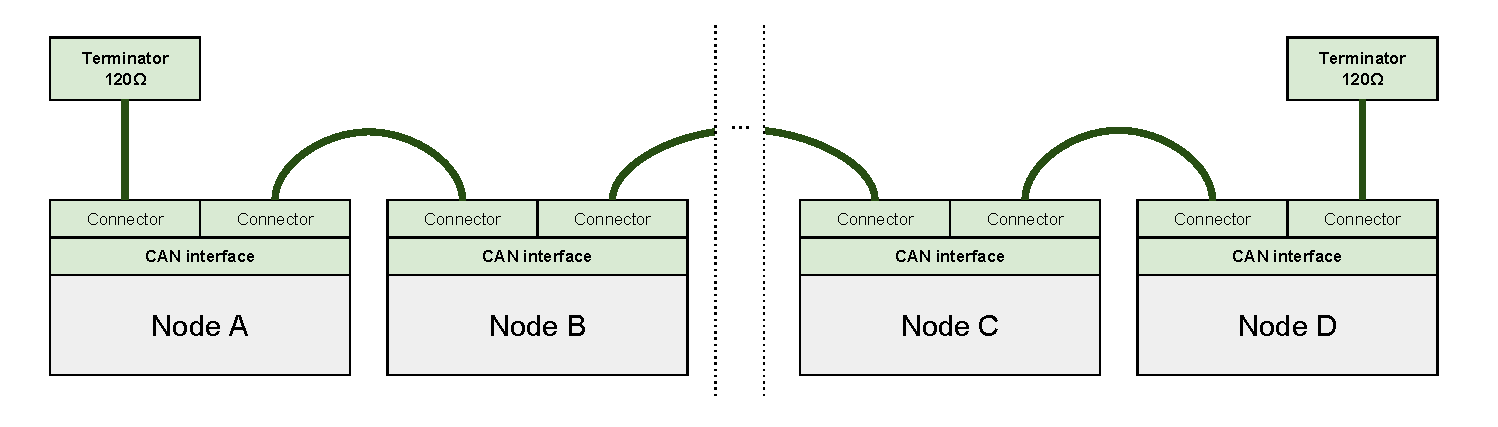
\includegraphics[width=1\textwidth]{can_daisy_chain}
    \caption{CAN bus interconnection diagram.
    \label{can_daisy_chain}}
\end{figure}

\subsubsection{Characteristics}

\begin{ZubaxTableWrapper}{UAVCAN Micro (JST GH) standard connector pinout}
    \begin{ZubaxWrappedTable}{|l X X[2]|}
        Pin no. & Type            & Function\\
        1       & Power           & +5 V power supply output and/or pass-trough\tnote{a}\\
        2       & Input/output    & CAN High\\
        3       & Input/output    & CAN Low\\
        4       & Ground          & Power \& signal ground\\
    \end{ZubaxWrappedTable}
	\begin{tablenotes}
	    \item[a] Power output can be enabled/disabled by setting the configuration parameter \CfgRef{can.power+on}.
	\end{tablenotes}
\end{ZubaxTableWrapper}

\begin{ZubaxTableWrapper}{CAN bus interface characteristics}
	\begin{ZubaxWrappedTable}{|c X|c c c|c|}
		Symbol  & Parameter                                 & Min  & Typ  & Max  & Unit \\
		        & Bit rate                                  & 10   &      & 1000 & Kbps \\
		        & Positive-going input threshold voltage    &      & 750  & 900  & mV \\
		        & Negative-going input threshold voltage    & 500  & 600  &      & mV \\
		        & Differential output voltage, dominant     & 1.5  & 2.0  & 3.0  & V \\
		        & Differential output voltage, recessive    & -120 & 0    & 12   & mV \\
		        & Inter-connector current pass-through\tnote{a}& -1&      & 1    & A \\
		        & Connector resistance during the device's lifetime && 30 & 50   & $\text{m}\Omega$ \\
		        & CAN bus power output voltage\tnote{b}     & $V_\text{supply}-$0.4
		                                                    & $V_\text{supply}-$0.3
		                                                    & $V_\text{supply}$
		                                                    & V \\
		        & CAN bus power output current              & -1   &      & 0.3  & mA \\
		        & Resistance of the embedded CAN terminator & 113  & 120  & 127  & $\Omega$ \\
	\end{ZubaxWrappedTable}
	\begin{tablenotes}
	    \item[a] The limit is imposed by the PCB.
	    \item[b] CAN power supply voltage is a function of the input supply voltage and
	             the voltage drop in the CAN power switch circuit.
	             The latter is dependent on the CAN power supply current.
	\end{tablenotes}
\end{ZubaxTableWrapper}

\subsection{USB}\label{sec:usb}

The device implements a full-speed USB 2.0 port with the standard CDC ACM interface
(also known as ``virtual serial port'').
The device features driverless compatibility with all major operating systems
(Windows, GNU/Linux, Mac OS).\footnote{Get more knowledge and helpful tips at \url{https://kb.zubax.com}.}

The physical connector type is USB micro B (which is one of the most common device-side USB connector types).

\subsubsection{Identification}

Babel will report the following properties to the USB host:
\begin{itemize}
    \item Vendor ID -- 0x1D50
    \item Product ID -- 0x60C7
    \item Vendor string -- \verb|Zubax Robotics|
    \item Device description string -- \verb|Zubax Babel|
    \item Device ID -- the 128-bit globally unique device ID (section \ref{sec:product_identification})
                       as a hexadecimal string
\end{itemize}

\subsection{Dronecode debug port}\label{sec:dronecode_debug_port}

The device features a Dronecode debug port interface available via the standard
Dronecode Debug Mini connector (DCD-Mini)\footnote{\url{https://wiki.dronecode.org/workgroup/connectors/start}}.
This port can be conveniently used with the \href{https://kb.zubax.com/x/iIAh}{Zubax Dronecode Probe},
or any other UART-capable hardware with a compatible connector.

The physical location of the connector is documented in the section \ref{sec:mechanical}.

The Dronecode debug port provides access to the UART and JTAG/SWD interfaces;
the latter is mostly useful for OEM applications and for using Babel as a development board.

\subsubsection{UART interface}

The baud rate can be changed by setting the configuration parameter \CfgRef{uart.baudrate}.
New baud rate settings take effect immediately.

The following parameters of the UART interface are fixed and cannot be changed by the user:
\begin{itemize}
    \item Word size -- 8 bit
    \item Parity control -- none
    \item Stop bits -- 1 bit
\end{itemize}

\subsubsection{SWD interface}

The SWD interface is a standard debug interface implemented in many ARM cores.
Please refer to the specialized literature for additional information.

Information about the use of Babel in OEM applications is provided in the section \ref{sec:oem_applications}.

The recommended SWD adapter for use with Babel is the \href{https://kb.zubax.com/x/iIAh}{Zubax Dronecode Probe}.

\subsubsection{Characteristics}

\begin{ZubaxTableWrapper}{Dronecode Debug Mini standard connector pinout}
    \begin{ZubaxWrappedTable}{|l X X X[2]|}
        Pin no. & Type            & Name                & Comment\\
        1       & Power           & TPWR                & +5 V power supply input/output\\
        2       & Output          & UART\_TX            & \\
        3       & Input           & UART\_RX            & Pulled up with a resistor\\
        4       & Input/Output    & SWDIO               & For OEM \& development use\\
        5       & Input           & SWDCLK              & For OEM \& development use\\
        6       & Ground          & GND                 & Power \& signal ground\\
    \end{ZubaxWrappedTable}
\end{ZubaxTableWrapper}

\begin{ZubaxSimpleTable}{Dronecode debug port characteristics}{|c X|c c c|c|}
	Symbol  & Parameter                                 & Min  & Typ    & Max         & Unit \\
                & Supported UART baud rates                 & 2400 & 115200 & 3\,000\,000 & baud/s \\
                & Low-level input voltage                   & -0.3 & 0      & 1.6         & V\\
                & High-level input voltage                  & 2.1  & 3.3    & 5.5         & V\\
                & Low-level output voltage                  & 0    & 0      & 0.5         & V\\
                & High-level output voltage                 & 2.8  & 3.3    & 3.4         & V\\
                & Source/sink current via data pins         &      &        & 10          & mA\\
                & UART RX pull up resistance                & 30   & 40     & 50          & $\text{k}\Omega$\\
	        & Connector resistance during device lifetime &    & 20     & 40          & $\text{m}\Omega$\\
\end{ZubaxSimpleTable}

\subsection{SMD pads}\label{sec:smd_pads}

Babel exposes a set of SMD pads which facilitate the following applications of the device:
\begin{itemize}
    \item Programmable CAN module for OEM applications.
          Babel can be directly soldered into a larger PCB using the exposed SMD pads.
    \item CAN development board.
          Standard 2.54\,mm connectors can be soldered to the SMD pads in order to make the device compatible with
          standard prototyping breadboards.
\end{itemize}

Information about the use of Babel in OEM applications is provided in the section \ref{sec:oem_applications}.
The pinout specification for the SMD pads is provided on the figure \ref{fig:pinout}.

\begin{ZubaxSimpleTable}{SMD signal pad characteristics}{|c X| c c c | c | }
    Symbol & Parameter                       & Min  & Typ & Max & Unit \\
           & Low-level input voltage         & -0.3 & 0   & 1.6 & V \\
           & High-level input voltage        & 2.1  & 3.3 & 5.5 & V \\
           & Low-level output voltage        & 0    & 0   & 0.5 & V \\
           & High-level output voltage       & 2.8  & 3.3 & 3.4 & V \\
           & Source/sink current (magnitude) &      &     & 10  & mA \\
\end{ZubaxSimpleTable}

\section{Product identification}\label{sec:product_identification}

This section documents the device properties that are reported in response to identification requests,
such the CLI command \verb|zubax_id| (section \ref{sec:cli_command_zubax_id}).

The product ID string is reported as ``\verb|com.zubax.babel|''.
The prefix ``\verb|com.zubax.|'' is shared by many of the products designed by Zubax Robotics.

Every manufactured device has a globally unique 128-bit ID (UID) that cannot be changed.

Every manufactured device is equipped with a certificate of authenticity,
which is a function of, among other things, the UID and the product ID of the device.
Please refer to the web resources provided by Zubax Robotics to learn more about the certificate of authenticity
and how it can be used to verify the authenticity of products.

\section{Geometry and pinout}\label{sec:mechanical}

The figure \ref{fig:drawing} documents the basic mechanical characteristics of Zubax Babel,
such as the placement of connectors and mounting holes.
The pinout of the SMD pads and other connectors is shown on the figure \ref{fig:pinout}.

\begin{figure}[hbtp]
	\centerline{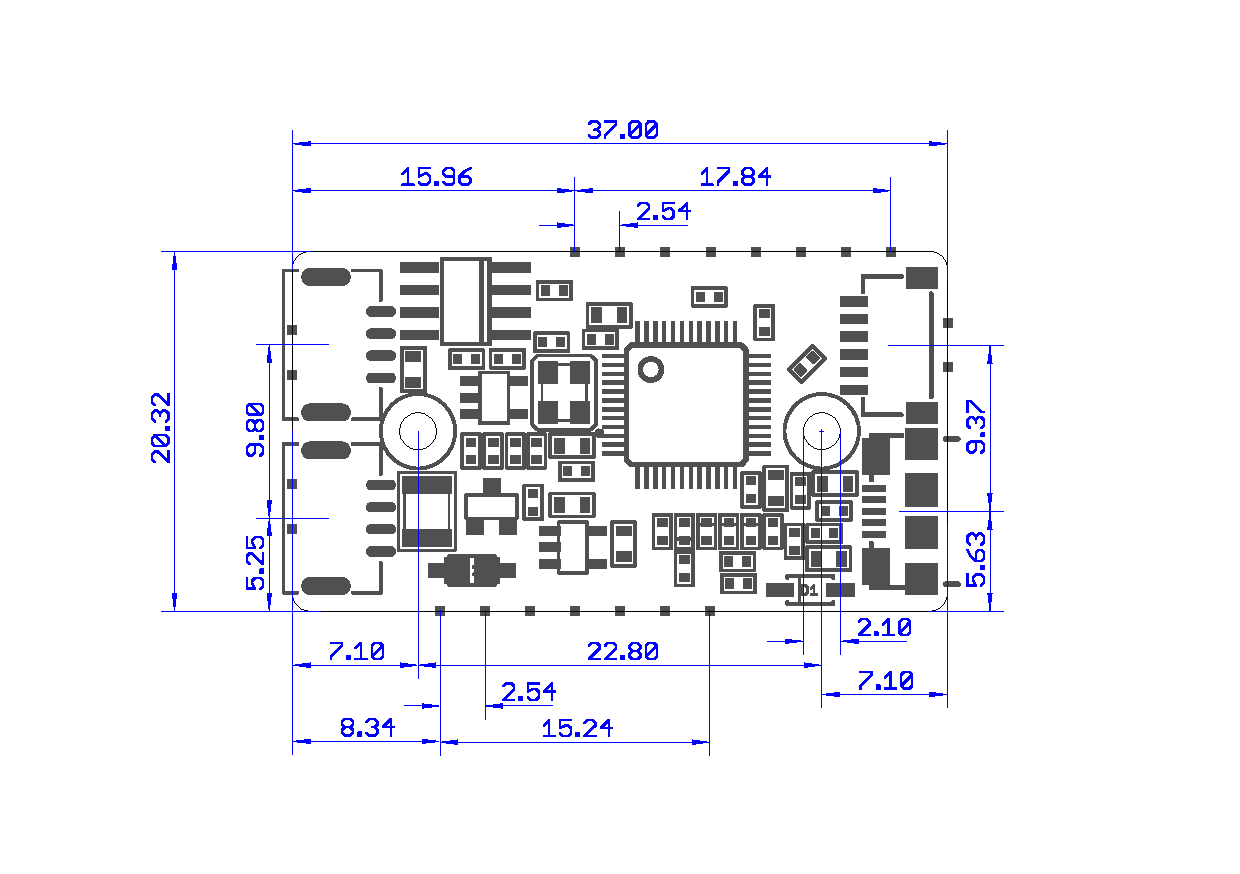
\includegraphics[width=1.2\textwidth]{babel_dimensions}}
	\caption{Physical dimensions of Babel.\label{fig:drawing}}
\end{figure}

\begin{figure}[hbtp]
	\centerline{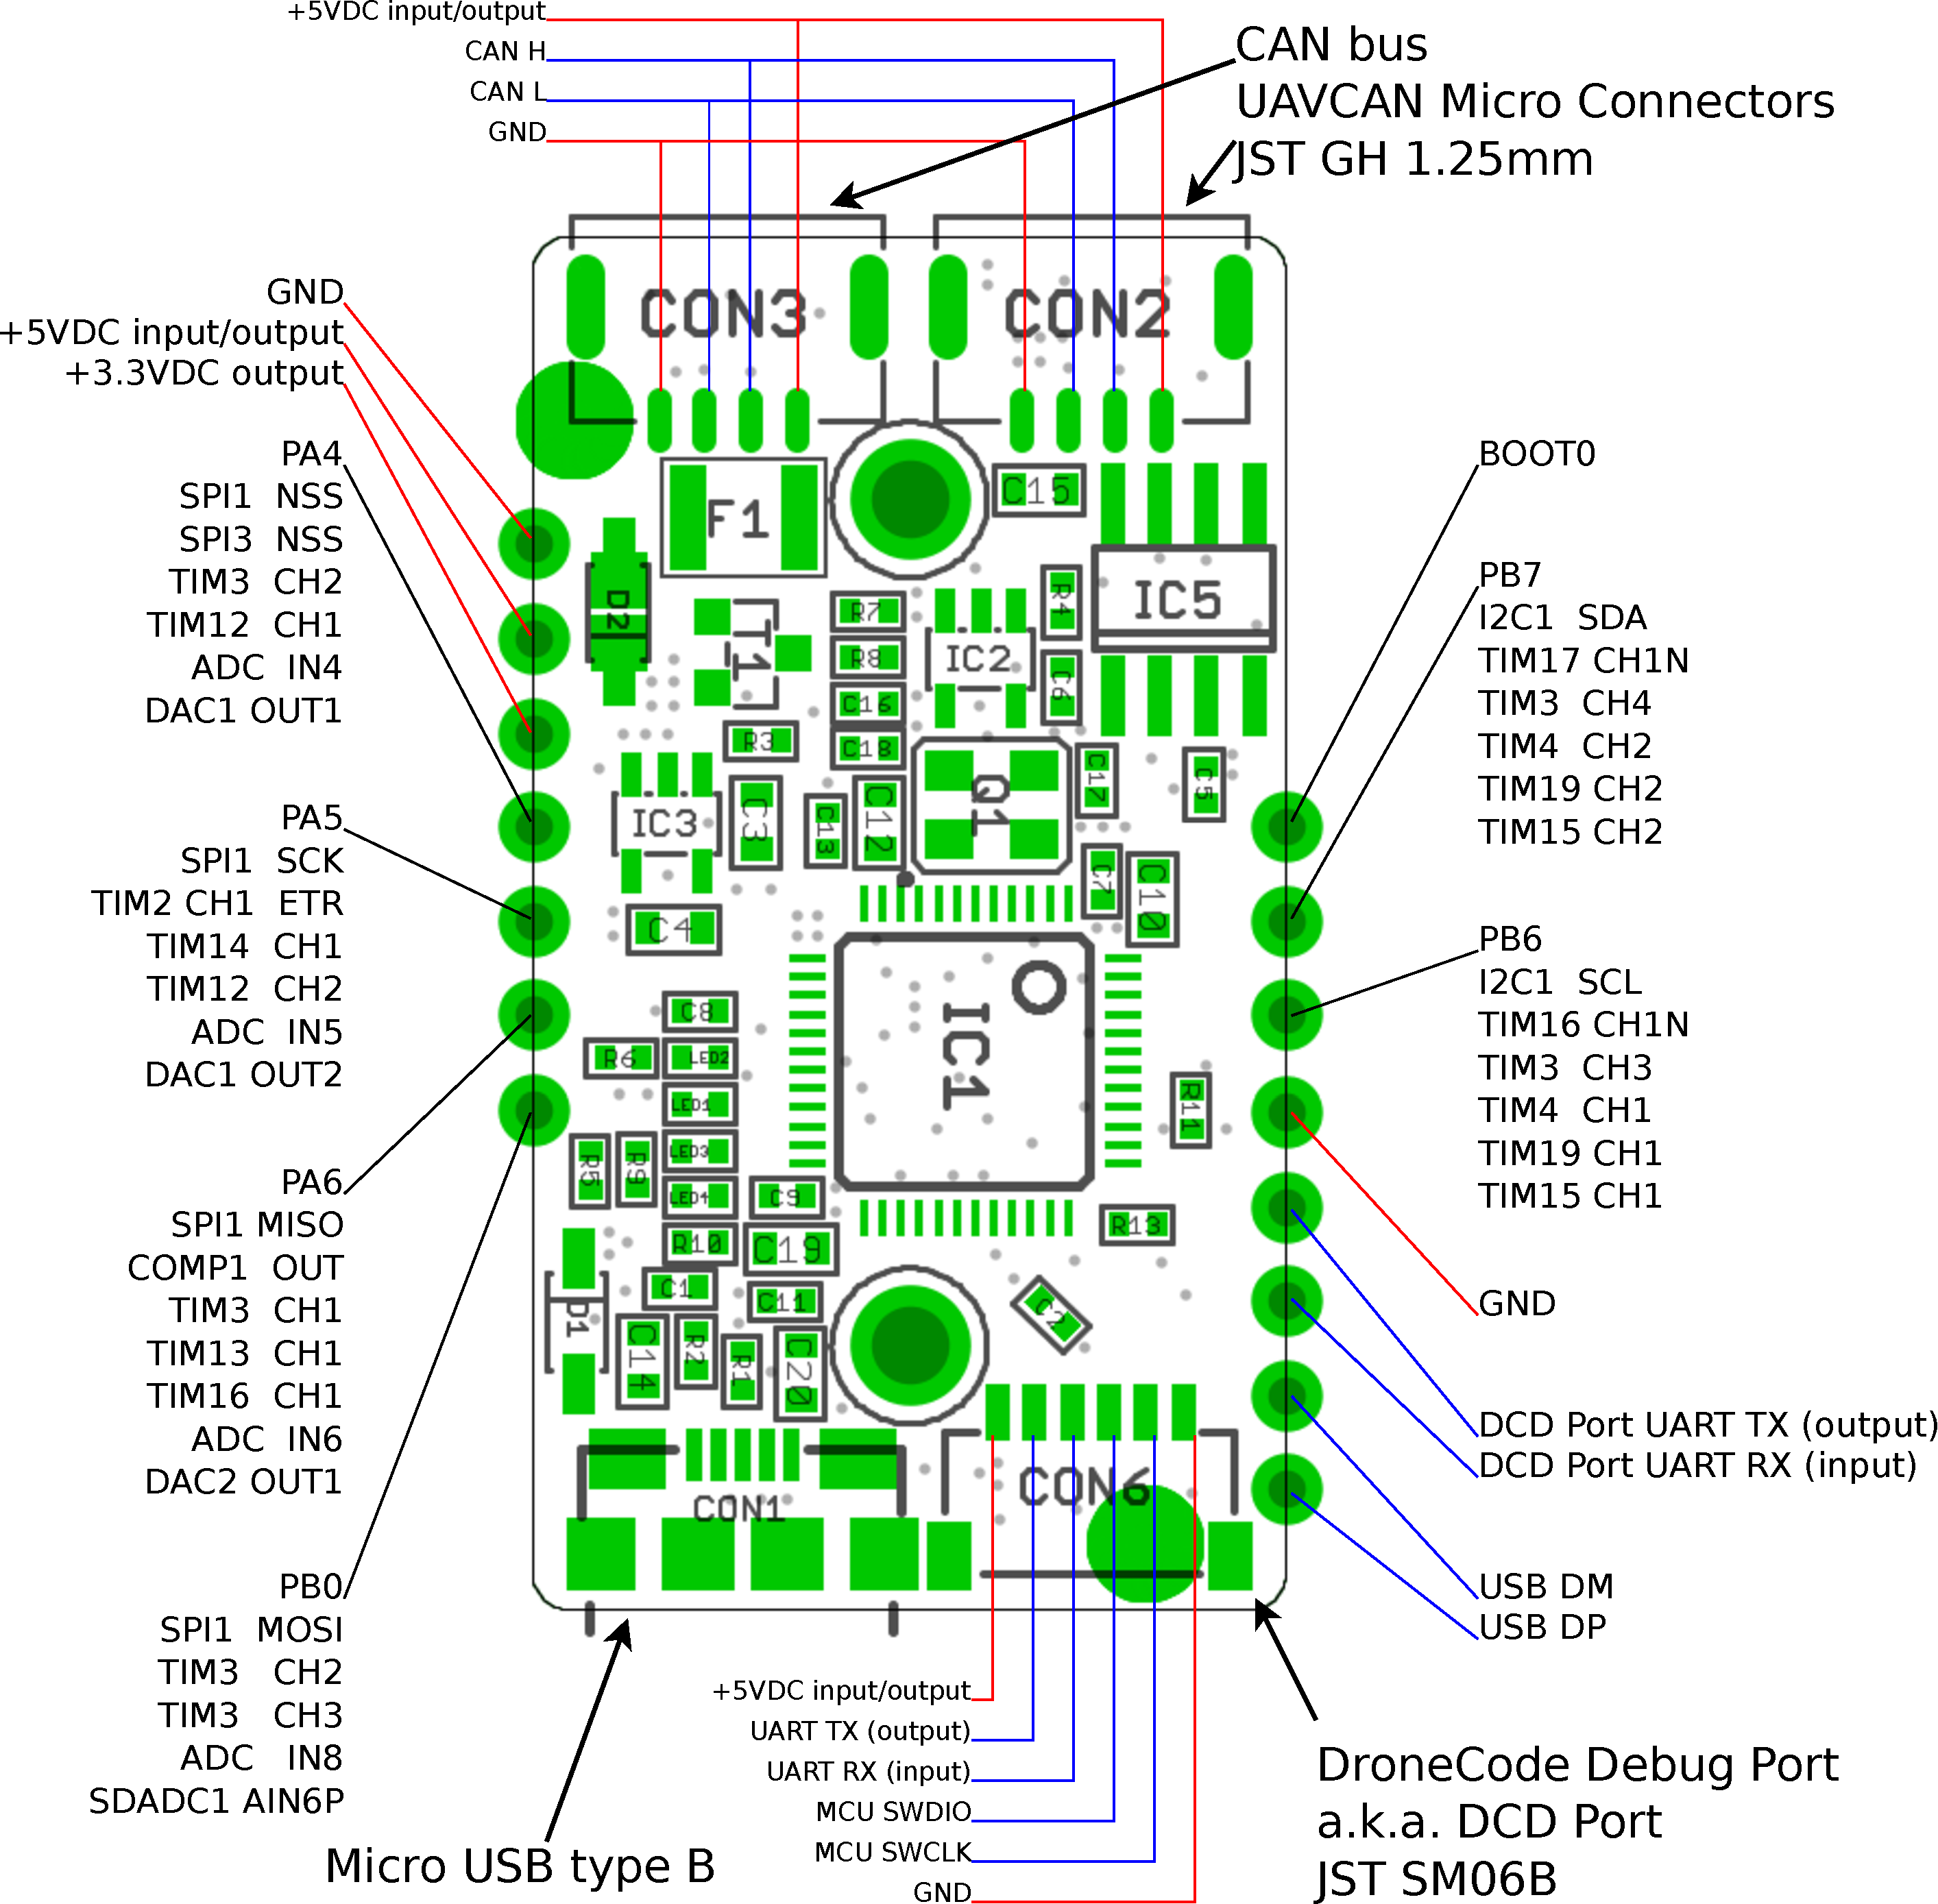
\includegraphics[width=1\textwidth]{pinout_annotated}}
	\vspace{2em}
	\caption{Babel pinout.\label{fig:pinout}}
\end{figure}

\chapter{Operating principles}

\section{Overview}

Babel keeps its CAN controller disabled by default in order to ensure that no unnecessary
interference with the CAN bus is introduced.
The CAN controller is enabled only if the host has requested Babel to open the data tunnel.
This is reviewed in more detail in the section \ref{sec:slcan}.

When opening the data tunnel, it is possible to explicitly specify the desired bit rate of the CAN bus.
If the CAN bit rate was not specified explicitly, Babel will use the value stored in the parameter
\CfgRef{can.bitrate}.
If the bit rate was specified explicitly, the parameter value will be automatically updated.

When the tunnel is opened, all of the buffers become flushed (i.e. cleared)
and the interface statistic counters get reset.
An attempt to open the tunnel when it is already opened is interpreted as if there was an implicit
close command before the tunnel is re-opened again.

Babel runs a single instance of an SLCAN protocol handler that can be attached either to the
USB CDC ACM interface (virtual serial port) or to the physical UART interface.
By default, the UART interface is used.
If Babel detects that the USB interface is connected to a USB host,
it disconnects the SLCAN protocol handler from the UART port and attaches it to the USB CDC ACM port.
The reverse happens when the USB port becomes disconnected.
It is therefore impossible to use both USB and UART interfaces at the same time concurrently.

\section{Start up and initialization}

Immediately after powering on, the device starts the embedded bootloader (described in detail in the section
\ref{sec:bootloader}).
The bootloader awaits for external commands for a few seconds.
If no commands requesting it to download a new firmware image or to wait longer were received,
and if a valid application (i.e. firmware) was found in the ROM,
the bootloader starts the application.
If no valid application is found in the ROM, the bootloader will wait for commands forever.

\section{LED indicators}

\newcommand{\LEDX}{{\rule{0.4em}{0.8em}}}
\newcommand{\LEDO}{{\rule{0.4em}{0.1em}}}

\newcommand{\ShowColor}[1]{{\color{#1}\rule{2em}{0.8em}}}

Babel is equipped with four separate LED indicators that reflect the current state of the device.
Their functions are summarized in the table \ref{table:led_indicators}.

\begin{ZubaxSimpleTable}{LED indicators}{|l l X|}\label{table:led_indicators}
    Color                     & Name               & Behavior \\
    \ShowColor{red} Red       & CAN power LED      & Glows when the CAN bus power output is enabled. \\
    \ShowColor{orange} Orange & CAN terminator LED & Glows when the CAN bus termination resistor is enabled. \\
    \ShowColor{blue} Blue     & Status LED         & See table \ref{table:status_led_behavior}. \\
    \ShowColor{green} Green   & CAN traffic LED    & Blinks once if at least one CAN frame was successfully
                                                     transmitted or successfully received in the last
                                                     25~milliseconds. Glows steadily when the intensity of CAN
                                                     traffic is higher than 40 frames per second.
                                                     The function of this LED is different while the bootloader
                                                     is running; see the section \ref{sec:bootloader}. \\
\end{ZubaxSimpleTable}

The behavior of the status LED is more complex than that of other indicators.
It is specified in the table \ref{table:status_led_behavior}.
Observe that there is one special mode that is used while the embedded bootloader is running.
The bootloader is documented separately in the section \ref{sec:bootloader}.

\begin{ZubaxSimpleTable}{Status LED behavior}{|l l X|}\label{table:status_led_behavior}
    Status & LED pattern (step 50 ms) & LED behavior \\

    Bootloader is running
    & {\color{blue}
       \LEDX\LEDX\LEDX\LEDX\LEDX\LEDX\LEDX\LEDX\LEDX\LEDX\LEDX\LEDX\LEDX\LEDX\LEDX\LEDX\LEDX\LEDX\LEDX\LEDX}
    & Glowing continuously.
      In this mode, the CAN traffic LED behaves as described in the section \ref{sec:bootloader}. \\

    CAN channel closed
    & {\color{blue}
       \LEDO\LEDO\LEDO\LEDO\LEDO\LEDO\LEDO\LEDO\LEDO\LEDO\LEDO\LEDO\LEDO\LEDO\LEDO\LEDO\LEDO\LEDO\LEDO\LEDO}
    & Turned OFF \\

    CAN channel open, normal operation
    & {\color{blue}
       \LEDX\LEDO\LEDO\LEDO\LEDO\LEDO\LEDO\LEDO\LEDO\LEDO\LEDO\LEDO\LEDO\LEDO\LEDO\LEDO\LEDO\LEDO\LEDO\LEDO}
    & Blinking 1 Hz \\

    CAN channel open, error passive
    & {\color{blue}
       \LEDX\LEDO\LEDO\LEDO\LEDO\LEDX\LEDO\LEDO\LEDO\LEDO\LEDX\LEDO\LEDO\LEDO\LEDO\LEDX\LEDO\LEDO\LEDO\LEDO}
    & Blinking 4 Hz \\

    CAN channel open, bus off
    & {\color{blue}
       \LEDX\LEDO\LEDX\LEDO\LEDX\LEDO\LEDX\LEDO\LEDX\LEDO\LEDX\LEDO\LEDX\LEDO\LEDX\LEDO\LEDX\LEDO\LEDX\LEDO}
    & Blinking 10 Hz \\
\end{ZubaxSimpleTable}

\chapter{SLCAN protocol}\label{sec:slcan}

\section{Introduction}

The SLCAN protocol (also known as LAWICEL protocol) is a quasi-standard protocol designed for
tunneling of CAN data (such as CAN frames, commands, and adapter status information)
via serial links (such as UART or USB virtual serial ports).

Babel implements all of the mandatory SLCAN commands,
so that its compatibility with third party software products that rely on SLCAN is ensured.
A brief recap of the standard SLCAN commands implemented in third-party products can be found
in the appendix \ref{appendix:slcan_api_overview}.

SLCAN is an ASCII text-based protocol, where the data is exchanged in blocks.
A block may contain only printable ASCII characters.

The end of a block is marked either with the ASCII carriage return character (\verb|\r|, code 13),
which is interpreted as a positive acknowledgement (ACK);
or the ASCII bell character (\verb|\a|, code 7),
which is interpreted as a negative acknowledgement (NACK).

A block begins with a well-defined character which indicates the kind of information the block is carrying;
in this description we're going to refer to this character as \emph{Block ID}.

The protocol defines three types of data blocks:

\begin{description}
    \item[Command] Blocks of this type are sent from the host to the adapter.
    \item[Response] Blocks of this type are sent from the adapter to the host
          as a reaction to a command. All commands provide exactly one response, unless stated otherwise.
    \item[Notification] Blocks of this type are generated by the adapter asynchronously.
\end{description}

All commands and notifications are always terminated with the ACK character (\verb|\r|).
A response will be terminated with ACK if the corresponding command has been executed successfully,
and with NACK if the command has failed or if the command could not be understood by the adapter.

Babel also implements an extension on top of the SLCAN protocol that allows the host to execute
arbitrary CLI commands over the same serial link that is used by SLCAN.
This feature is documented in the section \ref{sec:slcan_cli_extensions}.

Note that some commands alter the configuration parameters of the adapter.
All parameters are automatically stored in a non-volatile memory,
and their values are restored automatically whenever the adapter is turned on.
The section \ref{sec:configuration_parameters} provides an in-depth description of the configuration parameters
and their non-volatile storage.

The SLCAN interface can be exposed either via USB or via UART, but not both at the same time.
Babel connects the SLCAN interface to the USB virtual serial port as long as it is connected to a USB host.
When the USB interface is disconnected, the SLCAN interface is available via UART.

A high quality host-side implementation of the SLCAN protocol in Python can be found in the
\href{http://uavcan.org/Implementations/Pyuavcan/}{PyUAVCAN library} (MIT software license).

\section{SLCAN commands}

\subsection{CAN controller configuration commands}

\begin{ZubaxSimpleTable}{CAN controller configuration commands}{|l l X|}
    Block ID   & Arguments                 & Purpose \\

    \texttt{S} & Section \ref{sec:slcan_can_bit_rate_interpretation}
                                           & Set the CAN bit rate. The CAN bit rate will be stored in the
                                             configuration parameter \CfgRef{can.bitrate}. \\

    \makecell[lt]{\texttt{O}\\\footnotesize{(capital o)}}
               & None                      & Open CAN channel in normal mode; re-open if already open.
                                             The bit rate value will be taken from \CfgRef{can.bitrate}. \\

    \texttt{L} & None                      & Open CAN channel in silent mode (listen only); re-open if already open.
                                             The bit rate value will be taken from \CfgRef{can.bitrate}.
                                             Section \ref{sec:slcan_silent_mode}. \\

    \makecell[lt]{\texttt{l}\\\footnotesize{(lowercase L)}}
               & None                      & Open CAN channel in normal mode with loopback enabled;
                                             re-open if already open.
                                             The bit rate value will be taken from \CfgRef{can.bitrate}. 
                                             Section \ref{sec:slcan_loopback_mode}. \\

    \texttt{C} & None                      & Close CAN channel; do nothing if the channel is not open. \\

    \texttt{M} & Any                       & This command is not applicable to Babel,
                                             it is implemented only for compatibility reasons.
                                             Arguments are not validated. \\

    \texttt{m} & Any                       & See \texttt{M}.
\end{ZubaxSimpleTable}

All commands return ACK (\verb|\r|) on success and NACK (\verb|\a|) on failure.
Commands that are implemented only for compatibility always report success.

\subsubsection{CAN bit rate configuration}\label{sec:slcan_can_bit_rate_interpretation}

The command \verb|S| accepts a non-negative decimal number which represents the desired CAN bit rate.
If the channel is open, changes in the bit rate configuration will not take effect until it is re-opened again.
The values are interpreted as specified in the table \ref{table:slcan_can_bit_rate_interpretation}.

\begin{ZubaxSimpleTable}{CAN bit rate setting interpretation}{|l X|}\label{table:slcan_can_bit_rate_interpretation}
    Value     & Interpretation, bit/s \\ 
    0         & 10000 \\
    1         & 20000 \\
    2         & 50000 \\
    3         & 100000 \\
    4         & 125000 \\
    5         & 250000 \\
    6         & 500000 \\
    7         & 800000 \\
    8         & 1000000 \\
    Any other & The number is interpreted as-is, no additional conversion is performed.\\
\end{ZubaxSimpleTable}

\subsubsection{Silent mode}\label{sec:slcan_silent_mode}

When the channel is open in the silent mode,
the adapter configures its CAN controller in silent mode as well.
This mode ensures that the adapter will not interfere with the CAN bus,
regardless of the physical state of the interface (e.g. the controller will not confirm
received CAN frames; transmission of any CAN frames, including error frames, will never take place).

In silent mode, all outgoing CAN frames are ignored by the adapter.
CAN frames received from the bus are processed as usual.

\subsubsection{Loopback mode}\label{sec:slcan_loopback_mode}

When the channel is open with loopback enabled,
all transmitted frames will be immediately sent back to the host
after they were successfully delivered to the CAN bus.

If the SLCAN flags are enabled, loopback frames will be marked with an appropriate flag.
More information on SLCAN flags is provided in the section \ref{sec:slcan_notifications}.

\subsection{CAN frame transmission commands}

The following documentation uses the specified below notation to document the arguments of SLCAN commands:
\begin{description}
    \item[i] A hexadecimal digit that encodes the identifier of the current CAN frame.
    \item[d] A hexadecimal digit that encodes the DLC (data length code) of the current CAN frame.
    \item[*] An arbitrary sequence of useful bytes encoded as a hexadecimal string.
             For example, the sequence \verb|0110FF| encodes the following sequence of three bytes:
             1, 16, 255.
\end{description}

In SLCAN, hexadecimal digits can use both uppercase and lowercase Latin letters;
therefore, the complete set of characters that may occur in a hexadecimal number is as follows:
\verb|0123456789| \verb|abcdef| \verb|ABCDEF|.

\begin{ZubaxTableWrapper}{CAN frame transmission commands}
    \begin{ZubaxWrappedTable}{|l l l X|}
        Block ID   & Argument format     & Transmitted frame & Example of a complete SLCAN block \\

        \texttt{T} & \texttt{iiiiiiiid*} & Data frame with 29-bit ID
                                         & \texttt{T0123456780102030405060708\textbackslash{}r}\\

        \texttt{t} & \texttt{iiid*}      & Data frame with 11-bit ID
                                         & \texttt{t7FF0\textbackslash{}r}\\

        \texttt{R} & \texttt{iiiiiiiid}  & RTR frame with 29-bit ID\tnote{a}
                                         & \texttt{R1234f00d8\textbackslash{}r}\\

        \texttt{r} & \texttt{iiid}       & RTR frame with 11-bit ID\tnote{a}
                                         & \texttt{r008\textbackslash{}r}\\
    \end{ZubaxWrappedTable}
    \begin{tablenotes}
        \item[a] RTR frames don't carry payload data.
    \end{tablenotes}
\end{ZubaxTableWrapper}

All of the above listed commands may generate the responses specified in the table 
\ref{table:slcan_transmission_responses}.

Note that if a frame could not be scheduled for transmission due to the TX buffer being full,
the adapter would still return success.
Use the SLCAN flags together with the loopback mode in order to be able to detect when outgoing frames are dropped
by the adapter.

\begin{ZubaxSimpleTable}{CAN frame transmission responses}{|l X|}\label{table:slcan_transmission_responses}
    Response                    & Meaning \\

    \texttt{Z\textbackslash{}r} & The frame has been processed successfully (for 29-bit ID). \\

    \texttt{z\textbackslash{}r} & The frame has been processed successfully (for 11-bit ID). \\

    \texttt{\textbackslash{}a}  & The adapter could not transmit the frame.
                                  Some of the possible reasons include: a malformed SLCAN block,
                                  the CAN channel is not open.\\
\end{ZubaxSimpleTable}

\subsection{Miscellaneous commands}

\begin{ZubaxSimpleTable}{Miscellaneous commands}{|l l X|}
    Block ID   & Arguments & Purpose \\

    \texttt{U} & Section \ref{sec:slcan_uart_baud_rate_configuration}
               & Set the UART baud rate. The UART baud rate will be stored in the configuration parameter
                 \CfgRef{uart.baudrate}. \\

    \texttt{Z} & \texttt{0} or \texttt{1}
               & Enable or disable the RX and loopback timestamping.
                 The provided value will be stored in the configuration parameter \CfgRef{slcan.timestamping+on}.\\

    \texttt{F} & None
               & Get and clear the status flags. \\ 

    \texttt{V} & None
               & Get the hardware and software version numbers. \\

    \texttt{N} & None
               & Get the 128-bit unique ID of the device as a hexadecimal string
                 (section \ref{sec:product_identification}). \\
\end{ZubaxSimpleTable}

\subsubsection{UART baud rate configuration}\label{sec:slcan_uart_baud_rate_configuration}

The command \verb|U| accepts a non-negative decimal number which represents the desired UART baud rate.

The changes will take effect shortly after the command is executed (typically within 100 milliseconds),
no reboot is necessary;
therefore, the host should adjust the baud rate of the serial port immediately after this command is executed.

The argument is interpreted as specified in the table \ref{table:slcan_uart_baud_rate_configuration}.

\begin{ZubaxSimpleTable}{UART baud rate setting interpretation}{|l X|}
\label{table:slcan_uart_baud_rate_configuration}
    Value     & Interpretation, baud/s \\
    0         & 230400 \\ 
    1         & 115200 \\
    2         & 57600 \\
    3         & 38400 \\
    4         & 19200 \\
    5         & 9600 \\
    6         & 2400 \\
    Any other & The number is interpreted as-is, no additional conversion is performed.
\end{ZubaxSimpleTable}

At least the following baud rates are supported by the UART interface:
2400, 9600, 19200, 38400, 57600, 115200 (this is the default), 230400, 460800, 921600, 1\,000\,000, 3\,000\,000.

\subsubsection{CAN frame timestamping}

The command \texttt{Z} can be used to enable and disable the CAN frame timestamping feature.

The state of the timestamping feature is kept in the configuration parameter \CfgRef{slcan.timestamping+on}.

The changes will take effect shortly after the command was executed (typically within 100 milliseconds),
no reboot is necessary.

\subsubsection{Reading and clearing the status flags}

The command \verb|F| produces the following response:
\begin{minted}[linenos=0]{text}
F??\r
\end{minted}
Where \verb|??| is a hexadecimal bit mask.
The meaning of each bit in the bit mask is documented in the table \ref{table:slcan_status_bit_mask}.
Bits that are not used should be ignored when processing the bit mask.

\begin{ZubaxSimpleTable}{Bits of the F bit mask}{|l l l X|}\label{table:slcan_status_bit_mask}
    Bit & $\text{2}^\text{Bit}$ & Name   & Meaning \\

    0   & 1              &               & Not used. \\

    1   & 2              &               & Not used. \\

    2   & 4              &               & Not used. \\

    3   & 8              & RX overrun    & The RX queue has overflowed at least once since the last
                                           invocation of the F command or since the channel was open. \\

    4   & 16             &               & Not used. \\

    5   & 32             & Error passive & The CAN error counters have exceeded the error passive limit
                                           (refer to the CAN bus specification for details). \\

    6   & 64             &               & Not used. \\

    7   & 128            & Bus off       & The CAN controller is in the bus off state
                                           (refer to the CAN bus specification for details).\\
\end{ZubaxSimpleTable}

\subsubsection{Requesting the version information}

The command \verb|V| produces the following response:
\begin{minted}[linenos=0]{text}
V????\r
\end{minted}
Where the fields are one-digit hexadecimal numbers with the following meanings, in that order:
\begin{itemize}
\item Hardware version, major.
\item Hardware version, minor.
\item Software version, major.
\item Software version, minor.
\end{itemize}

\section{SLCAN notifications}\label{sec:slcan_notifications}

Babel emits SLCAN notifications in the following cases:
\begin{itemize}
    \item A CAN frame is received.
    \item If loopback is enabled: a CAN frame has been successfully delivered to the bus.
\end{itemize}

The format of notifications is the same as for CAN transmission commands.

\begin{ZubaxSimpleTable}{SLCAN notifications}{|l l X|}
    Block ID   & Argument format     & Purpose \\
    \texttt{T} & \texttt{iiiiiiiid*} & Received or successfully transmitted a 29-bit data frame.  \\
    \texttt{t} & \texttt{iiid*}      & Received or successfully transmitted an 11-bit data frame. \\
    \texttt{R} & \texttt{iiiiiiiid}  & Received or successfully transmitted a 29-bit RTR frame.   \\
    \texttt{r} & \texttt{iiid}       & Received or successfully transmitted an 11-bit RTR frame.  \\
\end{ZubaxSimpleTable}

Obviously, notifications for transmitted frames will be emitted only if the channel is open in the loopback mode.

Frame notifications may be extended with the timestamp information and/or with flags,
depending on the values of the configuration parameters \CfgRef{slcan.timestamping+on}
and \CfgRef{slcan.flags+on}, respectively.

When timestamping is enabled, every emitted CAN frame notification will be extended with
four more hexadecimal characters containing the time, in milliseconds, when the frame was received.
The millisecond timestamp overflows every 60\,000 milliseconds (once a minute),
so the valid values lie in the range from 0 to 59\,999, inclusive.

The frame timestamp can be converted into the target clock domain, e.g. the monotonic clock of the host system,
using the Olson algorithm\footnote{
\href{https://files.zubax.com/products/com.zubax.babel/olson_sensor_synchronization.pdf}
{``A Passive Solution to the Sensor Synchronization Problem'', Edwin Olson, 2010}.}
(the timestamp synchronization feature in PyUAVCAN is based on the Olson algorithm as well).

In the loopback mode with timestamping enabled the loopback frame notifications will carry the timestamp of
the moment when they were delivered to the bus.

When SLCAN flags are enabled, frame notifications will be amended as listed below.
Note that flags are always added at the end of the block.
\begin{itemize}
    \item Loopback frames will be appended with the character \verb|L| at the end of the block.
          This flag allows the host to distinguish the frames received from the bus from the
          transmitted frames that were looped back.

    \item Other flags may be added in future revisions of the protocol.
\end{itemize}

For example, an outgoing frame \texttt{T12345678401234568} will be looped back as shown in the table
\ref{table:slcan_notification_examples}, depending on the configuration.

\begin{ZubaxSimpleTable}{SLCAN notification example}{|l l l X|}\label{table:slcan_notification_examples}
    Flags? & Timestamping? & Representation & Comment \\
    No     & No            & \texttt{T12345678401234568\textbackslash{}r}
                           & No changes. \\

    No     & Yes           & \texttt{T123456784012345680BED\textbackslash{}r}
                           & Transmission timestamp 3053 milliseconds. \\

    Yes    & No            & \texttt{T12345678401234568L\textbackslash{}r}
                           & Added flag \texttt{L}.\\

    Yes    & Yes           & \texttt{T123456784012345680BEDL\textbackslash{}r}
                           & Both of the above two, flag after the timestamp. \\
\end{ZubaxSimpleTable}

\section{CLI extensions}\label{sec:slcan_cli_extensions}

Babel implements a proprietary extension of the SLCAN protocol that allows it to run a conventional
CLI\footnote{Command line interface.} shell over the same serial port that is used for SLCAN communications,
while maintaining full compatibility with SLCAN.

A CLI command is a sequence of printable ASCII characters terminated with the
\verb|\r\n| sequence (ASCII codes 13, 10).
The first non-whitespace character of a CLI command sequence cannot be also a valid
SLCAN block ID\footnote{For example, ``\texttt{T12345678401234568}'' is not a valid CLI command,
but ``\texttt{fooT12345678401234568}'' is acceptable.}.
The last limitation is necessary to ensure that the adapter can unambiguously distinguish between
a CLI command and an SLCAN block at the time of reception of the first character.
The early detection of SLCAN blocks allows the protocol state machine to dispatch CAN frames with
minimal latencies.

Every CLI command returns a response that begins with the exact copy of the received command terminated with
\verb|\r\n|,
then followed by an arbitrary number of lines of text,
each terminated with \verb|\r\n|,
and finalized with the ASCII END-OF-TEXT character (code 3) immediately followed by the final
\verb|\r\n|.

For example, a command ``\verb|cfg   list  |'' (the excessive spaces were added for the purposes of demonstration)
may produce the following response (in this example, the non-printable characters are shown with escape sequences,
e.g. \verb|\r|):

\begin{minted}[linenos = false]{yaml}
cfg   list  \r\n
can.bitrate           = 1000000     [10000, 1000000] (1000000)\r\n
can.power_on          = 0           [0, 1] (1)\r\n
can.terminator_on     = 0           [0, 1] (1)\r\n
slcan.timestamping_on = 1           [0, 1] (1)\r\n
slcan.flags_on        = 0           [0, 1] (0)\r\n
uart.baudrate         = 115200      [2400, 3000000] (115200)\r\n
\x03\r\n
\end{minted}

Where \verb|\x03| is the ASCII END-OF-TEXT character.

The following properties of the protocol allow both the adapter and the host
distinguish SLCAN data from CLI data in real time:
\begin{itemize}
    \item CLI commands and their responses are terminated with \verb|\r\n| rather than plain \verb|\r|.
    \item A valid SLCAN command cannot be also a valid CLI command.
\end{itemize} 
A compliant SLCAN driver that is capable of dealing with CLI extensions with virtually zero performance penalty
can be found in the PyUAVCAN library.

CLI commands can be executed manually by connecting to the SLCAN port using a terminal emulator program.
In this case it is recommended to enable local echo in the terminal emulator program,
because the SLCAN protocol does not provide remote echo.

\subsection{CLI commands}

This section documents the implemented CLI commands and provides usage instructions for them.

\subsubsection{cfg}

This command provides access to the configuration parameter storage.
The configuration parameters and their non-volatile storage are described in detail in the chapter
\ref{sec:configuration_parameters}.

Syntax:
\begin{itemize}
    \item \verb|cfg list| - list all configuration parameters, their current values,
          acceptable value intervals, and default values.

    \item \verb|cfg save| - save the current configuration into the non-volatile storage.
          This command is redundant and normally need not be used,
          because firmware revisions starting from v1.1 commit all configuration
          into the non-volatile storage automatically upon modification.

    \item \verb|cfg erase| - erase the current configuration and reset the non-volatile memory to
          the factory defaults.

    \item \verb|cfg set <name> <value>| - assign the configuration parameter named \verb|<name>| the value
          \verb|<value>|. For example: \verb|cfg set foo 42|.
          The non-volatile storage will be updated automatically.
\end{itemize}

The syntax \verb|cfg list| prints one parameter per line, where the line is formatted as follows:

\verb|name = value [min, max] (default)|

The number of whitespaces between tokens may vary.

Floating point parameters are always reported with the point symbol (\verb|.|),
which allows one to distinguish them from integer and boolean typed parameters.

Boolean parameters are reported as integers, where 1 represents the logical true and
0 represents the logical false.
They can be distinguished from integer parameters by their minimum and maximum values being 0 and 1,
respectively.

Whenever a parameter is assigned a new value, the device verifies if the new value is within the
acceptable limits.
If it is, the new value is assigned. Otherwise, the old value is retained.
Afterwards the device prints out the resulting value of the parameter in the following format:

\verb|name = value|

The number of whitespaces between tokens may vary.

The response can be used to check whether the new value was accepted by the device or not.

\subsubsection{zubax\textunderscore{}id}\label{sec:cli_command_zubax_id}

This command is available in all Zubax products that implement a command-line interface.
It reports the complete information identifying this particular product:
type, version information, make and model.
The information is printed in a machine-readable yet human-friendly
YAML\footnote{\url{https://en.wikipedia.org/wiki/YAML}} format.

An example output is shown in the following listing.
The meaning of each well-defined field is explained in the table \ref{zubax_id_fields_table}.
Note that the ordering of the fields is not guaranteed to be constant;
furthermore, additional fields may be added in future firmware revisions.

\begin{minipage}{0.9\textwidth} % A minipage is needed to avoid line breaks in the listing
\begin{minted}[linenos = false]{yaml}
product_id   : 'com.zubax.babel'
product_name : 'Zubax Babel'
sw_version   : '1.0'
sw_vcs_commit: 48923790
sw_build_date: Jun 20 2016
hw_version   : '1.0'
hw_unique_id : 'OAAyAA1XMkEzNjkgAAAAAA=='
hw_info_url  : http://device.zubax.com/device_info?uid=380032000D5732413336392000000000
hw_signature : 'SknsmA7XugU9pF/+NNOoU26Gdq9VvhO3O1Cw2qim17RXsU8yOISoKOdMIh4QIHtXr36sMfx
H397RlSNc0TtWDPOyA713z0k+v+ZY5PGXkRFiUfspnU/EJ8+r0url2dYp7NApx4lOklOgNgHrGCA6lPxA8UqoW
9jdqaASuqpFZKg='
\end{minted}
\end{minipage}

\begin{ZubaxSimpleTable}{Zubax ID fields}{|l X|}\label{zubax_id_fields_table}
Field name              & Meaning \\
\texttt{product\_id}    & Product type identifier string.
                          The same string is reported via UAVCAN as the node name string. \\
\texttt{product\_name}  & Human-readable product name. \\
\texttt{sw\_version}    & Firmware version number in the form ``major.minor''. \\
\texttt{sw\_vcs\_commit}& Firmware version short commit identifier (e.g. short git commit hash).
                          The abbreviation VCS stands for ``version control system''.
                          This number allows to pinpoint the exact revision of the firmware
                          that is currently running. \\
\texttt{sw\_build\_date}& Firmware build date in the form ``\texttt{mmm dd yyyy}''. \\
\texttt{hw\_version}    & Hardware version number in the form ``major.minor''. \\
\texttt{hw\_unique\_id} & The 128-bit unique ID of this specific hardware instance
                          (section \ref{sec:product_identification}).
                          The UID is represented either as a hexadecimal string, or as a Base64 encoded string.\\
\texttt{hw\_signature}  & The certificate of authenticity (CoA) of this specific hardware instance
                          encoded in a Base64 string.
                          If this data is missing, please inform Zubax Robotics as soon as possible. \\
\texttt{hw\_info\_url}  & Link to the web page that contains the test report, origin information,
                         traceability data, and other important information about this specific hardware
                         instance provided by the vendor.
                         If this data is missing, or if the linked web page is unreachable, please inform
                         Zubax Robotics as soon as possible. \\
\end{ZubaxSimpleTable}

\subsubsection{stat}

Returns a YAML dictionary containing the immediate state information of the adapter.

The statistic counters are reset every time the channel is opened.
Note that the statistics are kept intact after the channel is closed.

At least the following fields are reported in the output:
\begin{description}
    \item[open] Whether the CAN channel is open, either \verb|true| or \verb|false|.

    \item[state] One of the following: \verb|error_active|, \verb|error_passive|, \verb|bus_off|.
                 Please refer to the CAN protocol specification for the description of each state.

    \item[receive\_error\_counter] CAN receive error counter.
                                   Refer to the CAN protocol specification for more information.

    \item[transmit\_error\_counter] CAN transmit error counter.
                                    Refer to the CAN protocol specification for more information.

    \item[errors] The number of CAN protocol errors reported by the CAN controller hardware.

    \item[bus\_off\_events] The number of registered bus off events.

    \item[sw\_rx\_queue\_overruns] The number of overruns of the software RX queue.
                                   The software RX queue is positioned after the hardware RX queue.

    \item[hw\_rx\_queue\_overruns] The number of overruns of the hardware RX queue.
                                   The hardware RX queue is positioned before the software RX queue.

    \item[frames\_tx] The number of CAN frames successfully delivered to the bus.
                      Frames that were dropped due to overruns of the TX queue do not affect this statistic.

    \item[frames\_rx] The number of CAN frames received from the bus.
                      This statistic also includes frames that were lost due to overruns of the software RX queue.
                      Frames that were lost due to overruns of the hardware RX queue do not affect this statistic.

    \item[tx\_queue\_capacity] The capacity of the TX queue.

    \item[tx\_queue\_peak\_usage] The peak usage of the TX queue.

    \item[rx\_queue\_capacity] The capacity of the RX queue.

    \item[rx\_queue\_peak\_usage] The peak usage of the RX queue.

    \item[tx\_mailbox\_peak\_usage] The maximum number of TX mailboxes that were used simultaneously by the driver.
                                    The adapter uses an advanced algorithm of TX mailbox assignment in order to
                                    eliminate the inner priority inversion problem.

    \item[bus\_voltage] The voltage of the CAN bus power supply line, in volts.
\end{description}

An example output of this command is shown below:

\begin{minted}[linenos = false]{yaml}
open                  : true
state                 : error_active
receive_error_counter : 0
transmit_error_counter: 0
errors                : 0
bus_off_events        : 0
sw_rx_queue_overruns  : 0
hw_rx_queue_overruns  : 0
frames_tx             : 0
frames_rx             : 0
tx_queue_capacity     : 100
tx_queue_peak_usage   : 0
rx_queue_capacity     : 255
rx_queue_peak_usage   : 0
tx_mailbox_peak_usage : 0
bus_voltage           : 4.8
\end{minted}

\subsubsection{bootloader}

Reboots the device into the bootloader, where it will wait forever for commands.

This command reboots the device into the bootloader mode, described in the section \ref{sec:bootloader}.
It can be used to initiate a firmware update procedure over USB or UART.

\subsubsection{reboot}

Unconditionally reboots the device.

\chapter{OEM applications}\label{sec:oem_applications}

Besides its primary role of a USB-CAN or UART-CAN adapter tool,
Babel can be effectively used as an integral part of a larger system or a device:
either as a CAN adapter or, if loaded with a custom user-developed firmware,
in a completely different role.
These use cases are referred to as OEM applications.

Additionally, Babel can be used as a prototyping platform for quick development of CAN-dependent
(and especially UAVCAN-centric) applications.

More information about development of custom applications for Babel is available in the
Zubax Knowledge Base\footnote{\url{https://kb.zubax.com}}.

\section{SMD pads}

It is expected that OEM applications may require Babel to be installed on a custom PCB.
For this reason, Babel is given SMD pads spaced at the standard 2.54\,mm pitch.
Standard 2.54\,mm pin connectors can be soldered to the SMD pads in order to enable easy integration
with standard breadboards.

The signals that are routed to the pads are shown on the figure \ref{fig:pinout}.

\section{Custom applications}

Please refer to Zubax Knowledge Base for detailed information about development of custom applications.

Zubax Babel is based on the microcontroller STM32F373CBT6; its main characteristics are outlined below.

\begin{itemize}
    \item Core: ARM Cortex-M4F (with a hardware floating point unit) clocked at 72 MHz.
    \item Flash memory capacity: 128 KB.
    \begin{itemize}
        \item First 32 KB are occupied by the bootloader and some auxiliary persistent data.
        \item The following 94 KB are available for the user's application.
        \item Last 2 KB are reserved for non-volatile configuration storage.
    \end{itemize}
    \item RAM capacity: 24 KB.
    \begin{itemize}
        \item First 256 bytes are reserved for the bootloader.
        \item Remaining 24320 bytes are available for the user's application.
    \end{itemize}
\end{itemize}

Custom applications can be loaded either directly via the
SWD interface\footnote{We recommend Zubax Dronecode Probe for this task.},
in which case great care should be taken to not accidentally erase the bootloader;
or via the bootloader itself.
More information about the bootloader can be gathered in the section \ref{sec:bootloader}.

\chapter{Configuration parameters}\label{sec:configuration_parameters}

Configuration parameters are stored in a non-volatile memory on the adapter.

Some configuration parameters can be modified via dedicated SLCAN commands,
as described in the section \ref{sec:slcan}.

UAVCAN GUI Tool\footnote{\url{http://uavcan.org}} provides a convenient way of managing the
Babel's configuration parameters.

\begin{figure}[hbtp]
	\centerline{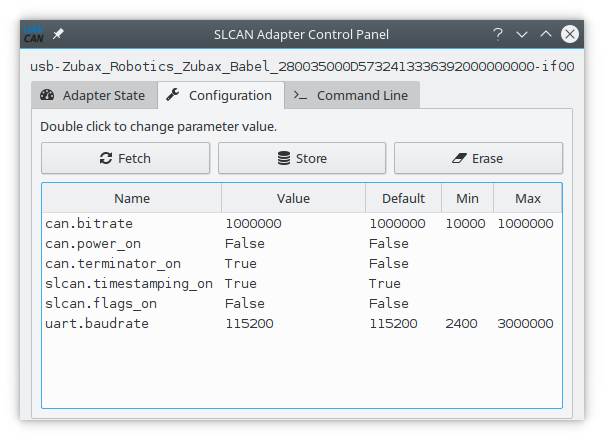
\includegraphics[width=0.7\textwidth]{uavcan_gui_tool_adapter_configuration}}
	\caption{Using the UAVCAN GUI Tool for configuration parameter management.}
\end{figure}

\section{Non-volatile configuration storage}

All configuration parameters are stored in a non-volatile memory
that retains its contents across power cycles.

Modification of any single parameter will trigger the device to commit all of them into the non-volatile
memory.\footnote{The auto-save feature is available since firmware v1.1.}

If the device is turned off while the configuration storage is being updated,
the stored configuration data may get damaged.

The stored configuration is read from the non-volatile memory once upon boot-up.
If the device detects that the stored configuration data has been damaged,
it will automatically revert to the factory default configuration.
Babel can always reliably detect damage of the stored configuration data,
so it is guaranteed that an invalid configuration can never be loaded.

\section{Firmware update considerations}

The configuration parameter sets of different firmware revisions may be incompatible with each other.
For instance, some configuration parameters may be added, removed, or their value intervals may be changed.

Babel always checks whether the stored configuration data is compatible with the current
firmware revision.
If it is detected that the stored configuration cannot be applied to the current version of the firmware,
the device will automatically revert to the factory default configuration.

Keep these considerations in mind when updating the firmware.

\section{Configuration parameter index}

The minimum, maximum, and default values provided in the table are shown for exemplary purposes only,
and they are \emph{not expected to be valid} for all firmware revisions that this document applies to.
Intervals and default values may change in newer revisions of the firmware or the hardware.

% name, SLCAN alias, takes effect at, min, max, default, note
\newcommand\CfgParamIndexEntry[7]{%
    \CfgDef{#1} & \footnotesize{#2} & \footnotesize{#3} & \footnotesize{\CfgListReferences{#1}} &
    \footnotesize{#4} & \footnotesize{#5} & \footnotesize{#6} & \footnotesize{#7}
    \tabularnewline
}%
\newenvironment{CfgParamIndex}[1]{%
    \begin{ZubaxTableWrapper}{#1}
    \setlength\tabcolsep{2.5pt}
    \begin{ZubaxWrappedTable}{@{} l c l l | c c c | X @{}}
    Name & \makecell[cb]{SLCAN\\alias} & \makecell[lb]{Takes\\effect at} & Pages & Min & Max & Def. & Description \\
}{%
    \end{ZubaxWrappedTable}
    \end{ZubaxTableWrapper}
}

\begin{CfgParamIndex}{Configuration parameter index}

\CfgParamIndexEntry{can.bitrate}{S}{channel open}{10\,000}{1\,000\,000}{1\,000\,000}
{CAN bus bit rate, in bit/s.}

\CfgParamIndexEntry{can.power+on}{}{immediately}{0}{1}{1}
{Enable CAN bus power output.}

\CfgParamIndexEntry{can.terminator+on}{}{immediately}{0}{1}{1}
{Enable the embedded CAN bus termination resistor.}

\CfgParamIndexEntry{slcan.timestamping+on}{Z}{immediately}{0}{1}{1}
{Time stamp all incoming and outgoing CAN frames.}

\CfgParamIndexEntry{slcan.flags+on}{}{immediately}{0}{1}{0}
{Enable flags for SLCAN notifications (SLCAN protocol extension).}

\CfgParamIndexEntry{uart.baudrate}{U}{immediately}{2400}{3\,000\,000}{115200}
{Baud rate of the UART port.}

\end{CfgParamIndex}

\chapter{Embedded bootloader}\label{sec:bootloader}

\section{Introduction}

Babel employs the Zubax Embedded Bootloader --
a highly robust open source bootloader designed for deeply embedded systems
that can update firmware over USB and serial port.
The bootloader also offers advanced integrity checking capabilities.

The bootloader starts immediately after the device has been powered on.
Having started, the bootloader checks if there is a valid application (i.e. firmware) that can be executed.
If there is one, the bootloader measures a 5 second timeout since the point of its initialization,
and once the timeout has expired, the bootloader starts the application,
unless an external entity has requested it to download a new application image or to wait longer.
If there is no valid application found (i.e. nothing to boot),
the bootloader will wait forever for commands.

The details about the supported communication interfaces are summarized in the table
\ref{table:bootloader_interfaces}.
Observe that this bootloader does not make use of the CAN bus interface.
As long as the bootloader is running, the CAN controller remains inactive
in order to avoid any interference with the CAN bus the device may be connected to.

The CAN power supply output and the CAN termination resistor remain inactive while the bootloader is running.

The bootloader is fully fault-tolerant.
If the update process fails at any point for any reason
(e.g. communication failure, power supply failure, and so on),
the device may end up with a damaged application.
The bootloader is able to recognize this condition and refuse to start the invalid application.
In order to recover from this state, the update process simply needs to be restarted.

As an additional safety measure, the bootloader uses a hardware watchdog timer that
allows it to abort applications that do not start properly.
This minimizes the chances of permanently incapacitating the device\footnote{Bricking.}
by uploading a dysfunctional application image.

\begin{ZubaxSimpleTable}{Bootloader communication interfaces}{| l | X | X[2] | X[2] |}
\label{table:bootloader_interfaces}
    Interface& Parameters                              & Protocol     & Note\\

    USB      & CDC ACM (virtual serial port)           & YMODEM, XMODEM, XMODEM-1K (autodetect)
                                                       & When USB is connected, the UART interface is inactive.\\

    UART     & 115200-8N1 (fixed)                      & Same as USB
                                                       & Available only while USB is disconnected.\\
\end{ZubaxSimpleTable}

\section{State machine}\label{sec:bootloader_state_machine}

The behavior of the bootloader if defined by a simple state machine documented on the figure
\ref{bootloader_state_machine}.
The table \ref{table:bootloader_states} summarizes the states.

\begin{figure}[!hbt]
	\centerline{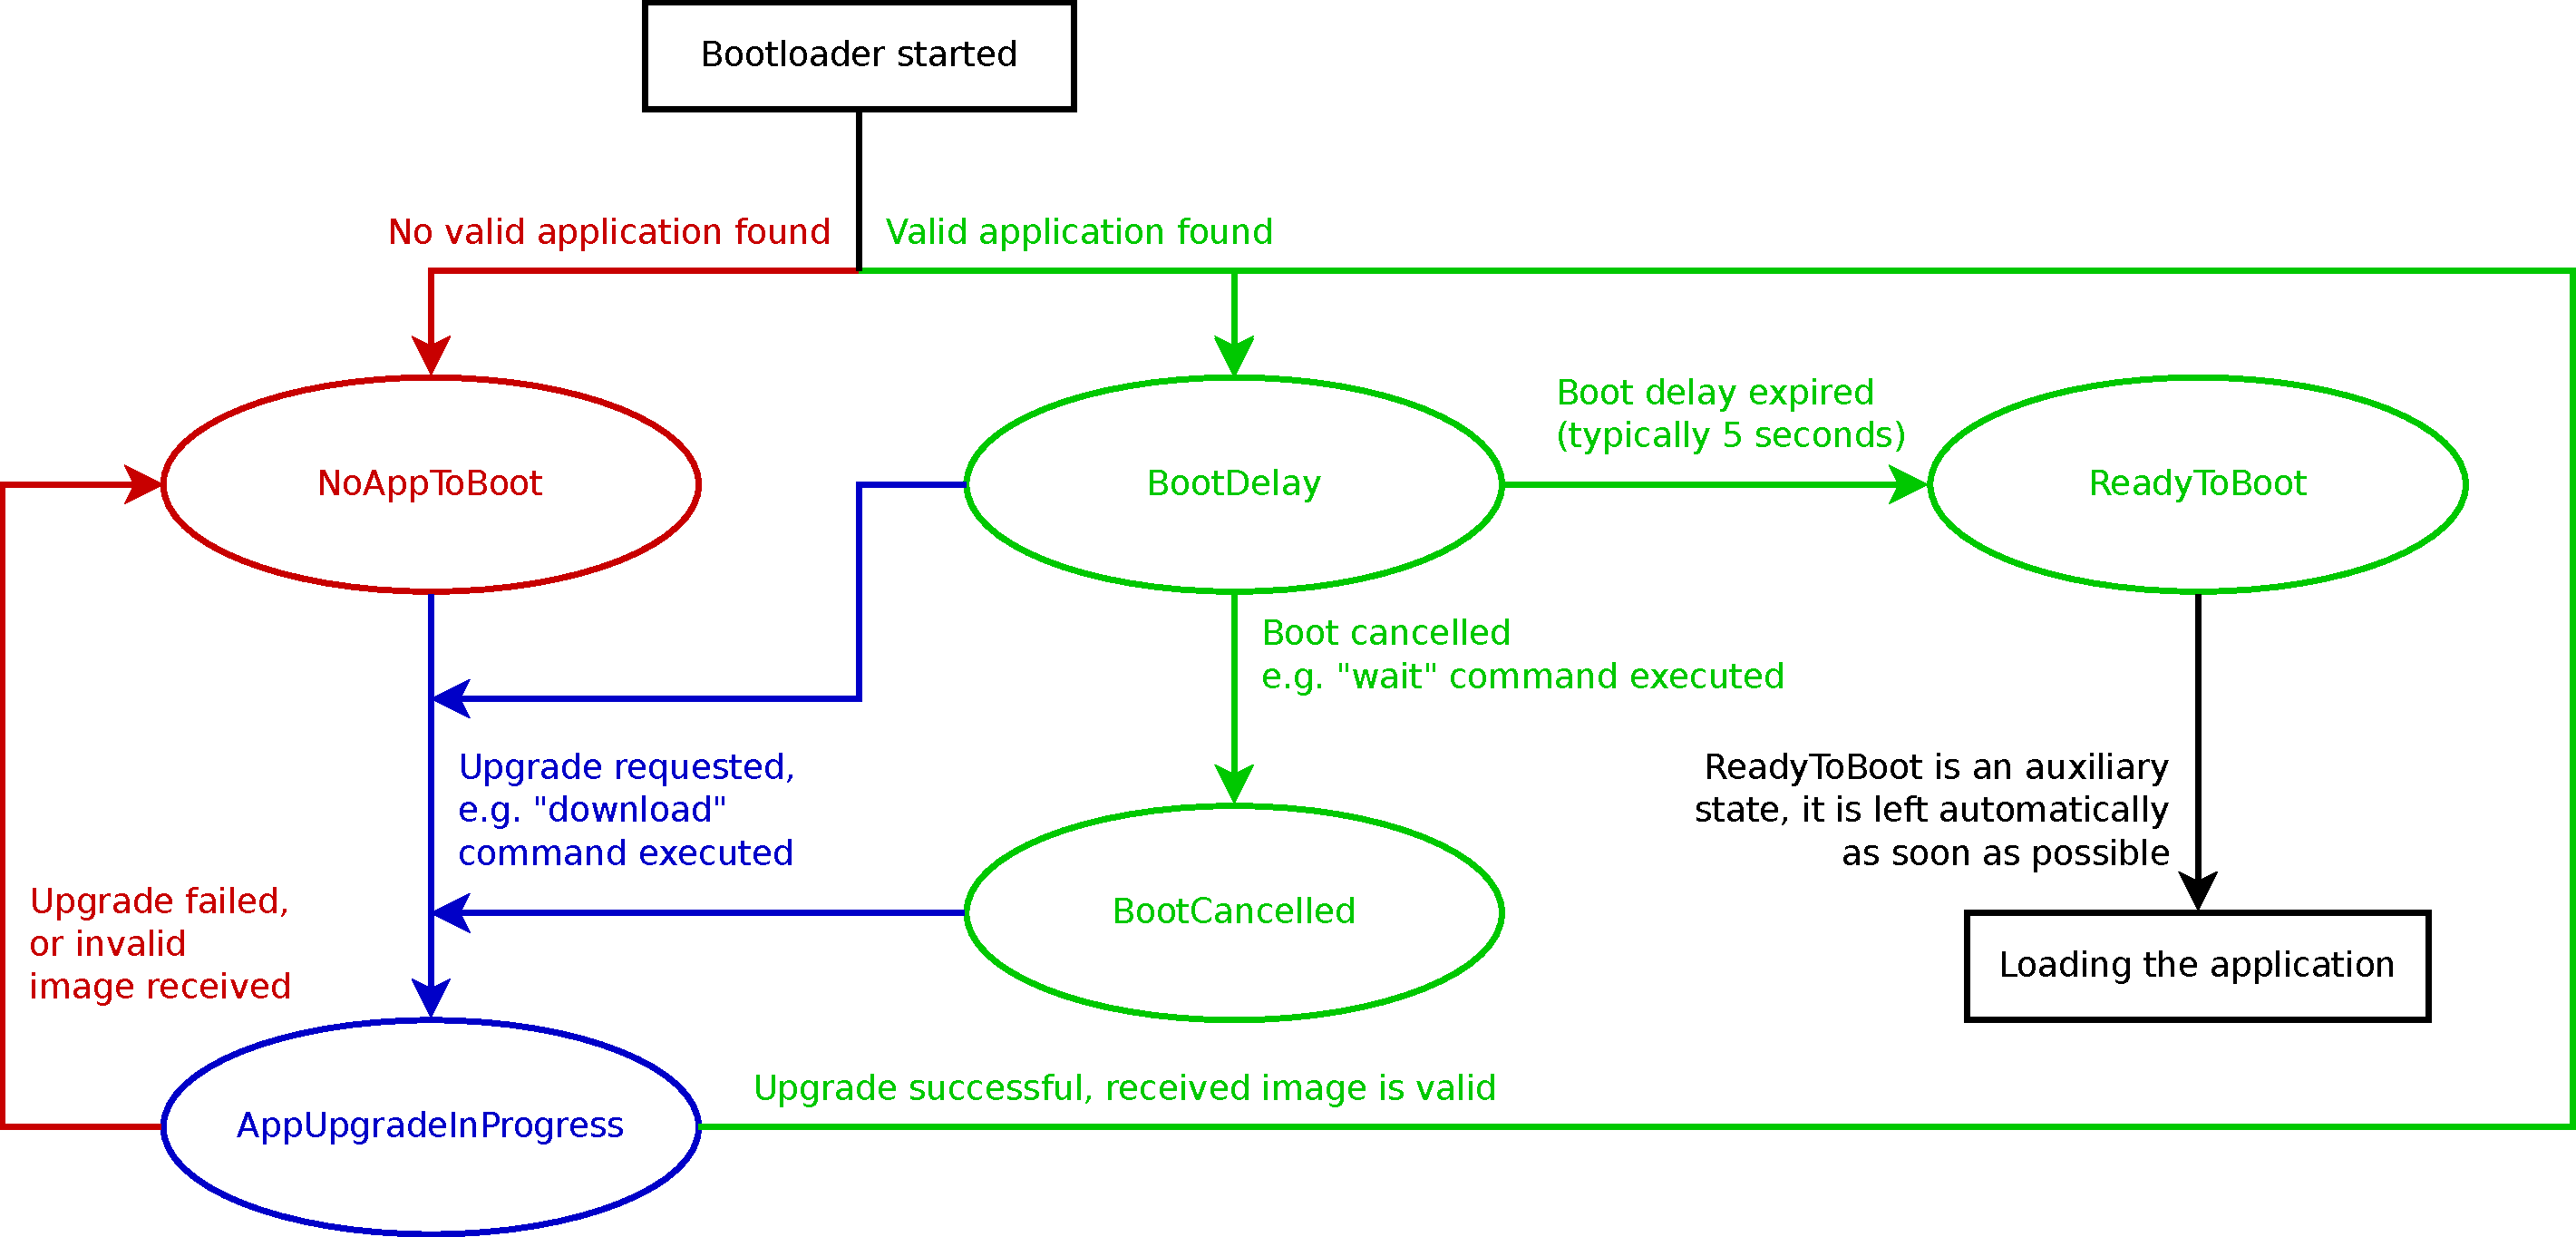
\includegraphics[width=\textwidth]{bootloader_state_machine}}
	\caption{Bootloader state machine.\label{bootloader_state_machine}}
\end{figure}

\begin{ZubaxSimpleTable}{Bootloader states}{|c l X|}\label{table:bootloader_states}
    ID & Name                 & Description \\

    0  & NoAppToBoot          & There is no valid application to boot;
                                the bootloader will be waiting for commands forever.\\

    1  & BootDelay            & The bootloader will start the application in a few seconds,
                                unless booting is canceled or an application update is requested.\\

    2  & BootCancelled        & There is a valid application to boot; however,
                                booting was canceled by an external command.\\

    3  & AppUpgradeinProgress & The application is currently being updated.
                                If interrupted, the bootloader will switch into
                                \textbf{NoAppToBoot} or \textbf{BootCancelled},
                                depending on whether there is a valid image after the interruption.\\
    
    4  & ReadyToBoot          & The application is about to be booted.
                                This state is very transient and is left automatically as soon as possible.\\
\end{ZubaxSimpleTable}

\section{LED indication}

While the bootloader is running, the LED indicators behave as described in this section.

The status LED (blue \ShowColor{blue}) is always on, which is the main indicator that the bootloader,
rather than the application (firmware), is currently running.

The CAN traffic LED (green \ShowColor{green}) displays one of the blinking patterns shown in the table 
\ref{table:bootloader_can2_led_behavior}, depending on which state the bootloader is in.

\begin{ZubaxSimpleTable}{Bootloader state indicated via the CAN traffic LED indicator}{|l l X|}
\label{table:bootloader_can2_led_behavior}
    Bootloader state         & LED pattern (step 50 ms) & LED behavior \\

    NoAppToBoot
    & {\color{green}
       \LEDX\LEDO\LEDX\LEDO\LEDX\LEDO\LEDX\LEDO\LEDX\LEDO\LEDX\LEDO\LEDX\LEDO\LEDX\LEDO\LEDX\LEDO\LEDX\LEDO}
    & Blinking 10 Hz (very quickly) \\

    BootDelay, ReadyToBoot
    & {\color{green}
       \LEDO\LEDO\LEDO\LEDO\LEDO\LEDO\LEDO\LEDO\LEDO\LEDO\LEDO\LEDO\LEDO\LEDO\LEDO\LEDO\LEDO\LEDO\LEDO\LEDO}
    & Turned off\\

    BootCancelled
    & {\color{green}
       \LEDX\LEDO\LEDO\LEDO\LEDO\LEDO\LEDO\LEDO\LEDO\LEDO\LEDO\LEDO\LEDO\LEDO\LEDO\LEDO\LEDO\LEDO\LEDO\LEDO}
    & Blinking 1 Hz, short pulses (50 ms)\\

    AppUpgradeInProgress
    & {\color{green}
       \LEDX\LEDX\LEDX\LEDX\LEDX\LEDX\LEDX\LEDX\LEDX\LEDX\LEDO\LEDO\LEDO\LEDO\LEDO\LEDO\LEDO\LEDO\LEDO\LEDO}
    & Blinking 1 Hz, long pulses (500 ms)\\
\end{ZubaxSimpleTable}

\section{Error codes}

The table \ref{table:bootloader_error_codes} provides descriptions for the well defined error codes
that can be reported by the bootloader.

\begin{ZubaxSimpleTable}{Bootloader error codes}{|r X|}\label{table:bootloader_error_codes}
    Code  & Description \\
        0 & Success.\\
        1 & Unknown error.\\
     9001 & Application ROM driver error: erase failed.\\
     9002 & Application ROM driver error: write failed.\\
    10001 & The current state of the bootloader does not permit the requested operation.\\
    10002 & Application image is too large for the device. Download has been aborted.\\
    10003 & Failed to write the next downloaded chunk of the application image into the ROM.\\
    20001 & X/YMODEM interface write has timed out.\\
    20002 & X/YMODEM retries exhausted.\\
    20003 & X/YMODEM protocol error.\\
    20004 & X/YMODEM transfer has been canceled by the remote.\\
    20005 & X/YMODEM remote has refused to provide the file.\\
    32767 & Unknown error.
\end{ZubaxSimpleTable}

\section{Interface selection}

Once started, the bootloader launches a CLI\footnote{Command line interface.} instance on the UART port.
If the bootloader detects that the USB interface became active (by virtue of being connected to a USB host),
it disconnects the CLI from UART, rendering the latter silent and unresponsive,
and connects the same CLI instance to the USB virtual serial port.
The CLI will remain available on the USB virtual serial port as long as the USB interface is active.
Shall the USB port become disconnected, the bootloader will switch the CLI back to UART.
The switching between USB and UART is fully automatic and happens on the fly.

\section{USB interface properties}

The USB interface will be detected by the host as CDC ACM (also known as virtual serial port).
This is a standard USB class that is supported by vast majority of operating systems out of the box,
no special drivers are required.

The bootloader reports the following properties to the USB host:
\begin{itemize}
    \item Vendor ID -- 0x1D50
    \item Product ID -- 0x60C7
    \item Vendor string -- \verb|Zubax Robotics|
    \item Device description string -- \verb|Zubax Babel Bootloader|
    \item Device ID -- the 128-bit globally unique device ID (section \ref{sec:product_identification})
                       as a hexadecimal string
\end{itemize}

\section{UART interface properties}

The UART interface has the following properties that cannot be changed:
\begin{itemize}
    \item Baud rate -- 115200
    \item Word size -- 8 bit
    \item Parity control -- none
    \item Stop bits -- 1
\end{itemize}

\section{CLI properties}

The CLI uses the CR-LF line ending sequence (\verb|\r\n|).
In order to avoid unintended side effects of exposing the bootloader's CLI when the
outer hardware expects an SLCAN interface,
the bootloader's CLI does not return any echo until the input of a valid command has been completed.

For example, entering a command \verb|zubax_id| will not produce any echo, until the command has been completed
with the \verb|\r\n| sequence.
As such, entering \verb|zubax_id\r\n| will return the echo followed by the command output.
Echo for invalid commands is never returned.

The delayed echo allows the bootloader to silently ignore all SLCAN traffic and other data it doesn't recognize.
Otherwise, the echo emitted by the bootloader could be misinterpreted by the connected hardware
as valid SLCAN data.

Due to the above considerations, the CLI does not offer any prompt.

\section{CLI commands}

This section documents the CLI commands that can be of interest to the end user.
Some commands that are not intended for use in production are intentionally omitted from this reference.

\subsection{reboot}

Restarts the bootloader normally.

\subsection{wait}

Instructs the bootloader to not boot the application automatically.

If the current state is \verb|BootDelay|, the state will be switched to \verb|BootCancelled|.
In all other states the command will have no effect.

\subsection{download}

Instructs the bootloader to start an YMODEM/XMODEM/XMODEM-1K receiver on the current serial link
and await for the remote host to begin transmission of the new application image file.

The bootloader will automatically detect which file transfer protocol to use.

According to the YMODEM specification, if no transfer was initiated by the host within one minute,
the command will exit with an error.
Possible error codes are defined in the table \ref{table:bootloader_error_codes}.

Note that while this command is running, the CLI will be unavailable,
because the same serial link will be temporarily occupied by the file transfer protocol.
Automatic switching between USB and UART is not available while the command is running.

See the section \ref{sec:bootloader_ymodem_implementation} for the detailed information about the implementation.

\subsection{zubax\textunderscore{}id}

This is a standard command documented in the section \ref{sec:cli_command_zubax_id}.
Its implementation in the bootloader, however, has a number of additional features.

The software version information provided in the output is obtained from the application that is
currently installed on the device.
If the bootloader could not find any installed application,
the software version fields will be omitted from the
output.\footnote{Version 1.0 of the bootloader used to employ a different convention where the application
version fields were using a different prefix: \texttt{fw\_} rather than \texttt{sw\_}.}

The version of the bootloader itself is reported via the following set of dedicated fields:
\begin{itemize}
    \item \verb|bl_version| -- bootloader version, major and minor, formatted as \verb|<major>.<minor>|
    \item \verb|bl_vcs_commit| -- bootloader version control system commit identifier as an integer number.
    \item \verb|bl_build_date| -- the build date of the bootloader.
\end{itemize}

An additional field named ``\verb|mode|'' is set to the string ``\verb|bootloader|''
to indicate that the bootloader is currently running rather than the application.

The table \ref{table:bootloader_zubax_id_fields} summarizes the fields reported by the bootloader.
Some extra fields may be reported as well,
which are not documented here because they are not designed for production use.

\begin{ZubaxSimpleTable}{Zubax ID fields}{|l X|}\label{table:bootloader_zubax_id_fields}
Field name              & Meaning \\

\texttt{product\_id}    & Product type identifier string.
                          The same string is reported via UAVCAN as the node name string. \\

\texttt{product\_name}  & Human-readable product name. \\

\texttt{mode}           & Set to the string ``\texttt{bootloader}'' to indicate that the bootloader is running. \\

\texttt{sw\_version}    & Application version number in the form ``major.minor''.
                          Omitted if the application could not be found. \\

\texttt{sw\_vcs\_commit}& Application version control system commit identifier.
                          Omitted if the application could not be found. \\

\texttt{hw\_version}    & Hardware version number in the form ``major.minor''. \\

\texttt{hw\_unique\_id} & The 128-bit unique ID of this specific hardware instance
                          (section \ref{sec:product_identification}).\\

\texttt{hw\_signature}  & The certificate of authenticity (CoA) of this specific hardware instance
                          encoded in a Base64 string.
                          If this data is missing, please inform Zubax Robotics as soon as possible. \\

\texttt{bl\_version}    & Bootloader version number in the form ``major.minor''. \\

\texttt{bl\_vcs\_commit}& Bootloader version control system commit identifier. \\
\end{ZubaxSimpleTable}

\subsection{state}

Prints the current state of the bootloader in the following form:
\begin{minted}[linenos=false]{text}
StateName (StateID)
\end{minted}
Where \verb|StateName| is the name of the current state as specified in the table \ref{table:bootloader_states},
and \verb|StateID| is the numerical identifier of the current state.

An example output is shown below:
\begin{minted}[linenos=false]{text}
BootCancelled (2)
\end{minted}

\section{YMODEM/XMODEM/XMODEM-1K implementation details}\label{sec:bootloader_ymodem_implementation}

YMODEM, XMODEM, and XMODEM-1K are simple and popular file transfer protocols designed by
Ward Christensen and Chuck Forsberg.
You can learn more about these protocols in the Zubax Knowledge Base at \url{https://kb.zubax.com/x/ZwAz}.
This section elaborates on the noteworthy implementation details specific to this application.

The \verb|download| command starts a multi-protocol receiver.
The receiver enters a loop where it emits the ASCII NAK character to the host,
prompting it to begin transmission of the application image file.
The receiver will emit NAK every 5 seconds until the host begins the transmission,
until the transfer initialization times out,
or until the host cancels the transmission, whichever happens first.
The transfer initialization timeout is set to 1 minute.

The receiver always uses the NAK character to initiate transfers rather than ``\verb|C|'',
which instructs the remote host to use the plain 8-bit checksum for data integrity checking
rather than CRC-16.
The data integrity guarantees offered by the plain 8-bit checksum algorithm are deemed sufficient,
because the data links are considered reliable enough,
and the application image itself is always protected by a strong CRC function.

Being compatible with three different protocols, the receiver supports the following options:
\begin{itemize}
    \item The host is free to send the zero block with the file metadata, as defined by YMODEM.
          The receiver will collect the file size information from the metadata packet and ignore the rest.
    
    \item The host is free to use either 256-byte or 1024-byte sized blocks, the receiver supports both.
          The former are defined by YMODEM and XMODEM, the latter are defined by YMODEM and XMODEM-1K.
\end{itemize}

Note that if the size of the application image file has not been provided,
the written image will be padded up to the size of the last data block.
This is acceptable, because the trailing bytes after the application image are
not used by any part of the system, and as such their contents can be arbitrary.
It is recommended, however, to fill the padding bytes with 0xFF,
in order to match the initial state of the ROM.

There is a large number of software products and scripts that support these file transfer protocols.
For instance, the popular program \verb|sz| (available on most GNU/Linux distributions) can be used as follows
(where \verb|$file| is the name of the application image file, and \verb|$port| is the name of the serial port):
\begin{minted}[linenos = false]{bash}
sz -vv --ymodem --1k \$file > \$port < \$port
\end{minted}
There are various GUI-based alternatives for Windows and Mac OS as well.

%
% BEGIN APPENDICES
%
\appendix
\chapter{Appendix: Third party SLCAN API implementations}\label{appendix:slcan_api_overview}

\begin{figure}[hbtp]
    \centering
	\centerline{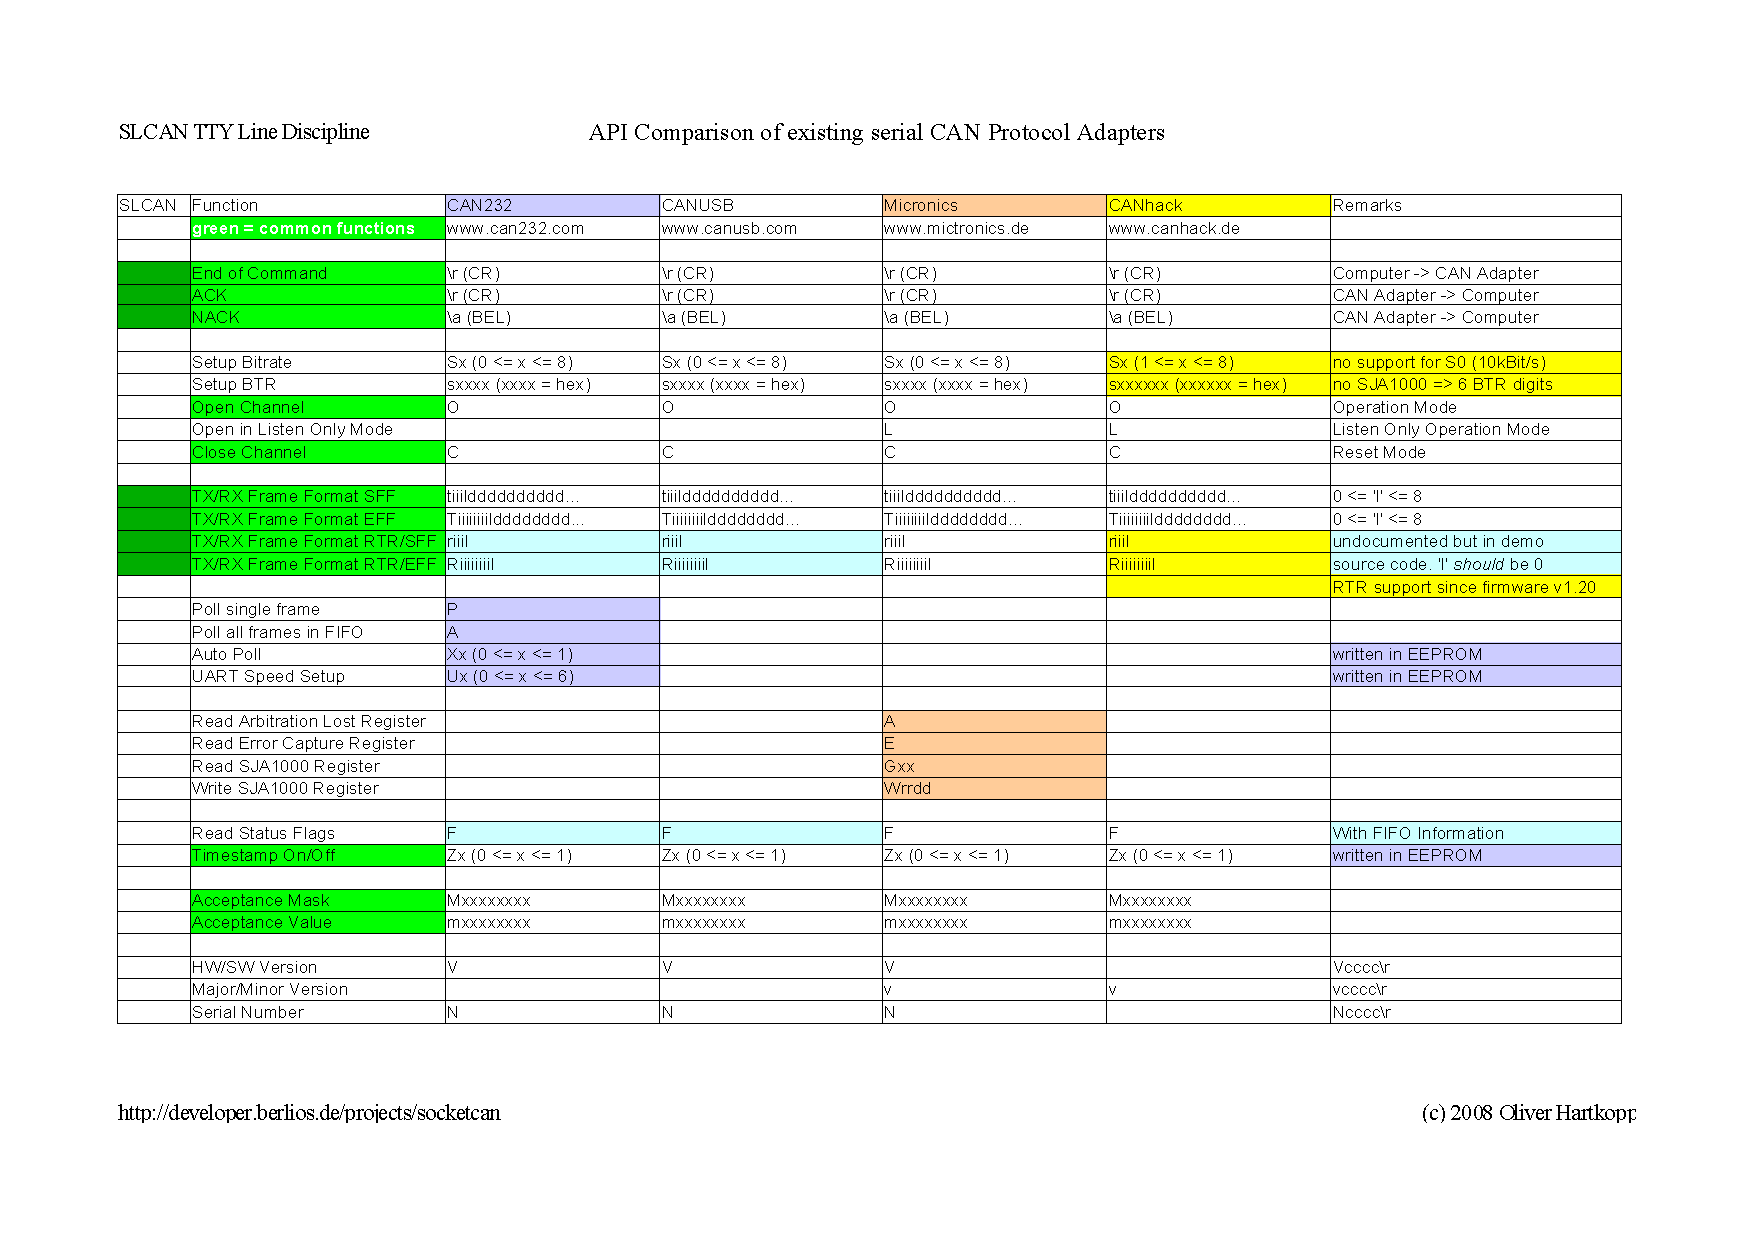
\includegraphics[width=1.2\textwidth]{Generic_SLCAN_API}}
	\caption{An overview of the SLCAN API implemented in various SLCAN-compatible adapters.
	\label{fig:Generic_SLCAN_API}}
	Prepared by Oliver Hartkopp (Linux SocketCAN project).
\end{figure}

\end{document}
